% Para utilizar este template siga o tutorial disponível em http://www.biblioteca.ufc.br/wp-content/uploads/2015/09/tutorial-sharelatex.pdf

%%%%%%%%%%%%%%%%%%%%%%%%%%%%%%%%%%%%%%%%%%%%%%%%%%%%%%%
%% Você deve criar uma conta no Overleaf. Depois,    %%
%% vá nas opções no canto esquerdo superior da tela  %%
%% e clique em "Copiar Projeto". Dê um novo nome pa- %%
%% ra o projeto.                                     %%
%%                                                   %%
%% Os principais desenvolvedores deste template são: %%
%%                                                   %%
%%            Ednardo Moreira Rodrigues              %%
%%       (Doutor em Engenharia Elétrica - UFC)       %%
%%                      &                            %%
%%            Alan Batista de Oliveira               %%
%%           (Engenheiro Eletricista - UFC)          %%
%%                                                   %%
%% Consultoria Bibliotecária                         %%
%%                                                   %%
%%  Versão 2016 - ShareLaTeX:                        %% 
%%                                                   %%
%% - Francisco Edvander Pires Santos;                %%
%% - Juliana Soares Lima;                            %%
%% - Izabel Lima dos Santos;                         %%
%% - Kalline Yasmin Soares Feitosa;                  %%
%% - Eliene Maria Vieira de Moura.                   %%
%%
%%  Versão 2019 - Overleaf:
%%  
%%  Biblioteca de Ciências Humanas: 
%% - Francisco Edvander Pires Santos;                %%
%% - Juliana Soares Lima;                            %%
%% - Eliene Maria Vieira de Moura;                   %%
%% - Edmundo Moreira de Sousa Filho.                 %%
%%                                                   %%
%% Biblioteca da FEAAC:                              %%
%% - Izabel Lima dos Santos;                         %%
%% - Kalline Yasmin Soares Feitosa;                  %%
%% - Kleber Lima dos Santos.                         %%
%%                                                   %%
%%  Biblioteca do Curso de Física:                   %%
%% - Aline Rodrigues de Lima Mendes;                 %%
%% - Maria de Jesus Silva dos Santos.                %%
%%                                                   %%
%%  Biblioteca Central do Campus do Pici:            %%
%% - Raquel da Silva Nascimento.                     %%
%%                                                   %%
%% Colaboradores                                     %%
%%                                                   %%
%% -Andrei Bosco Bezerra Torres                      %% 
%% (Professor - Sistemas e Mídias Digitais -         %%
%% Instituto Universidade Virtual - UFC)             %%
%% Tiago ALves Lima                                  %% 
%% (Aluno de Mestrado em Eng. Elétrica)              %%
%%                                                   %%
%% Grande parte do trabalho foi adaptado do template %%
%% da UECE elaborado por:                            %%
%% Thiago Nascimento  (UECE)                         %%
%% Project available on:                             %%
%% https://github.com/thiagodnf/uecetex2             %%
%%                                                   %%
%% "Dúvidas, esclarecimentos ou sugestões podem ser  %%
%% enviadas para o seguinte e-mail:                  %%
%%                                                   %%
%%             atendimentobch@ufc.br                 %%
%%                                                   %%
%% As últimas atualizações estão descritas no inicio %%
%% do arquivo "README.md".                           %%
%%                                                   %%
%%%%%%%%%%%%%%%%%%%%%%%%%%%%%%%%%%%%%%%%%%%%%%%%%%%%%%%

\documentclass[        
    a4paper,          % Tamanho da folha A4
    12pt,             % Tamanho da fonte 12pt
    chapter=TITLE,    % Todos os capitulos devem ter caixa alta
    section=Title,    % Todas as secoes devem ter caixa alta somente na primeira letra
    subsection=Title, % Todas as subsecoes devem ter caixa alta somente na primeira letra
    oneside,          % Usada para impressao em apenas uma face do papel
    english,          % Hifenizacoes em ingles
    spanish,          % Hifenizacoes em espanhol
    brazil,           % Ultimo idioma eh o idioma padrao do documento
    fleqn             % Comente esta linha se quiser centralizar as equacoes. Comente também a linha 65 abaixo
]{abntex2}

% Para utilizar este template siga o tutorial disponível em http://www.biblioteca.ufc.br/wp-content/uploads/2015/09/tutorial-sharelatex.pdf

%%%%%%%%%%%%%%%%%%%%%%%%%%%%%%%%%%%%%%%%%%%%%%%%%%%%%%%
%% Você deve criar uma conta no Overleaf. Depois,    %%
%% vá nas opções no canto esquerdo superior da tela  %%
%% e clique em "Copiar Projeto". Dê um novo nome pa- %%
%% ra o projeto.                                     %%
%%                                                   %%
%% Os principais desenvolvedores deste template são: %%
%%                                                   %%
%%            Ednardo Moreira Rodrigues              %%
%%       (Doutor em Engenharia Elétrica - UFC)       %%
%%                      &                            %%
%%            Alan Batista de Oliveira               %%
%%           (Engenheiro Eletricista - UFC)          %%
%%                                                   %%
%% Revisão:                                          %%
%%                                                   %%
%% - Francisco Edvander Pires Santos;                %%
%% - Juliana Soares Lima;                            %%
%% - Izabel Lima dos Santos;                         %%
%% - Kalline Yasmin Soares Feitosa.                  %%
%% - Eliene Maria Vieira de Moura;                   %%
%%                                                   %%
%% Colaboradores                                     %%
%%                                                   %%
%% -Andrei Bosco Bezerra Torres                      %% 
%% (Professor - Sistemas e Mídias Digitais -         %%
%% Instituto Universidade Virtual - UFC)             %%
%% Tiago ALves Lima                                  %% 
%% (Aluno de Mestrado em Eng. Elétrica)              %%
%%                                                   %%
%% Grande parte do trabalho foi adaptado do template %%
%% da UECE elaborado por:                            %%
%% Thiago Nascimento  (UECE)                         %%
%% Project available on:                             %%
%% https://github.com/thiagodnf/uecetex2             %%
%%                                                   %%
%% "Dúvidas, esclarecimentos ou sugestões podem ser  %%
%% enviadas para o seguinte e-mail:                  %%
%%                                                   %%
%%             atendimentobch@ufc.br                 %%
%%                                                   %%
%% As últimas atualizações estão descritas no inicio %%
%% do arquivo "README.md".                           %%
%%                                                   %%
%%%%%%%%%%%%%%%%%%%%%%%%%%%%%%%%%%%%%%%%%%%%%%%%%%%%%%%

% Importações de pacotes
\usepackage[utf8]{inputenc}                         % Acentuação direta
\usepackage[T1]{fontenc}                            % Codificação da fonte em 8 bits
\usepackage{graphicx}                               % Inserir figuras
\usepackage{amsfonts, amssymb, amsmath}             % Fonte e símbolos matemáticos
\usepackage{booktabs}                               % Comandos para tabelas
\usepackage{verbatim}                               % Texto é interpretado como escrito no documento
\usepackage{multirow, array}                        % Múltiplas linhas e colunas em tabelas
\usepackage{indentfirst}                            % Endenta o primeiro parágrafo de cada seção.
\usepackage{listings}                               % Utilizar codigo fonte no documento
\usepackage{xcolor}
\usepackage{microtype}                              % Para melhorias de justificação?
\usepackage[portuguese,ruled,lined]{algorithm2e}    % Escrever algoritmos
\usepackage{algorithmic}                            % Criar Algoritmos  
%\usepackage{float}       
% \usepackage{pdflscape}
% Utilizado para criação de floats
\usepackage{amsgen}
\usepackage{lipsum}                                 % Usar a simulação de texto Lorem Ipsum
%\usepackage{titlesec}                              % Permite alterar os títulos do documento
\usepackage{tocloft}                                % Permite alterar a formatação do Sumário
\usepackage{etoolbox}                               % Usado para alterar a fonte da Section no Sumário
\usepackage[nogroupskip,nonumberlist]{glossaries}   % Permite fazer o glossario

\usepackage[font=singlespacing,format=plain,justification=justified,skip=0pt,singlelinecheck = false]{caption}            % Altera o comportamento da tag caption

\usepackage[alf, abnt-emphasize=bf, recuo=0cm, abnt-etal-cite=2, abnt-etal-list=0, abnt-etal-text=it]{abntex2cite}  % Citações padrão ABNT
%\usepackage[bottom]{footmisc}                      % Mantém as notas de rodapé sempre na mesma posição
%\usepackage{times}                                 % Usa a fonte Times
%%%%%%%%%%%%%%%%%%% AVISO %%%%%%%%%%%%%%%%%%%%%%%%%%%%%%%%%%%%%%%%
%descomente as duas linhas abaixo para alterar o texto de Times New Roman para Arial:

%\usepackage{helvet}
%\renewcommand{\familydefault}{\sfdefault}  % Usa a fonte Arial              
%%%%%%%%%%%%%%%%%%%%%%%%%%%%%%%%%%%%%%%%%%%%%%%%%%%%%%%%%%%%%%%%%%

\usepackage{mathptmx}         % Usa a fonte Times New Roman			%\usepackage{lmodern}         % Usa a fonte Latin Modern
%\usepackage{subfig}          % Posicionamento de figuras
%\usepackage{scalefnt}        % Permite redimensionar tamanho da fonte
%\usepackage{color, colortbl} % Comandos de cores
%\usepackage{lscape}          % Permite páginas em modo "paisagem"
%\usepackage{ae, aecompl}     % Fontes de alta qualidade
%\usepackage{picinpar}        % Dispor imagens em parágrafos
%\usepackage{latexsym}        % Símbolos matemáticos
\usepackage{upgreek}         % Fonte letras gregas
\usepackage{appendix}         % Gerar o apendice no final do documento
\usepackage{paracol}          % Criar paragrafos sem identacao
\usepackage{lib/ufctex}	      % Biblioteca com as normas da UFC para trabalhos academicos
\usepackage{pdfpages}         % Incluir pdf no documento
\usepackage{amsmath}          % Usar equacoes matematicas

\usepackage{adjustbox}       % Pra ajustar tabela com \resizebox



\makeglossaries % Organiza e gera a lista de abreviaturas, simbolos e glossario
\makeindex      % Gera o Indice do documento         




\setlength{\mathindent}{0pt} %Complementa o alinhamento de equações para totalmente a esquerda.

%%%%%%%%%%%%%%%%%%%%%%%%%%%%%%%%%%%%%%%%%%%%%%%%%%%%%
%%                     ATENCAO                     %%
%%%%%%%%%%%%%%%%%%%%%%%%%%%%%%%%%%%%%%%%%%%%%%%%%%%%%
%  Qual e o nivel do trabalho academico que voce esta 
% escrevendo? Retire o simbolo "%" apenas de um dos 
% quatro topicos abaixo refente ao nível do seu traba
% -lho.

\trabalhoacademico{tccgraduacao}
%\trabalhoacademico{tccespecializacao}
%\trabalhoacademico{dissertacao}
%\trabalhoacademico{tese}

%%%%%%%%%%%%%%%%%%%%%%%%%%%%%%%%%%%%%%%%%%%%%%%%%%%%%

% Define se o trabalho e uma qualificacao
% Coloque 'nao' para versao final do trabalho

\ehqualificacao{nao}

% Remove as bordas vermelhas e verdes do PDF gerado
% Coloque 'sim' pare remover

\removerbordasdohyperlink{sim} 

% Adiciona a cor Azul a todos os hyperlinks

\cordohyperlink{nao}

%%%%%%%%%%%%%%%%%%%%%%%%%%%%%%%%%%%%%%%%%%%%%%%%%%%%%
%%         Informacao sobre a instituicao          %%
%%%%%%%%%%%%%%%%%%%%%%%%%%%%%%%%%%%%%%%%%%%%%%%%%%%%%

\ies{Universidade Federal do Ceará}
\iessigla{UFC}
\centro{Centro de Tecnologia}
\departamento{Departamento de Engenharia de Teleinformática}

%%%%%%%%%%%%%%%%%%%%%%%%%%%%%%%%%%%%%%%%%%%%%%%%%%%%%
%%        Informacao para TCC de Graduacao         %%
%%%%%%%%%%%%%%%%%%%%%%%%%%%%%%%%%%%%%%%%%%%%%%%%%%%%%

\graduacaoem{Engenharia De Computação}
\habilitacao{bacharel} % Ou licenciado(a)

% AVISO: Caso necessario alterar o texto de apresenta-
% cao da Especializacao, ir a pasta "lib", arquivo 
% "ufctex.sty" na linha 502.


%%%%%%%%%%%%%%%%%%%%%%%%%%%%%%%%%%%%%%%%%%%%%%%%%%%%%
%%     Informacao para TCC de Especializacao       %%
%%%%%%%%%%%%%%%%%%%%%%%%%%%%%%%%%%%%%%%%%%%%%%%%%%%%%

\especializacaoem{Yyyyyyyyy}

% AVISO: Caso necessario alterar o texto de apresenta-
% cao da Especializacao, ir a pasta "lib", arquivo 
% "ufctex.sty" na linha 507.

%%%%%%%%%%%%%%%%%%%%%%%%%%%%%%%%%%%%%%%%%%%%%%%%%%%%%
%%         Informacao para Dissertacao             %%
%%%%%%%%%%%%%%%%%%%%%%%%%%%%%%%%%%%%%%%%%%%%%%%%%%%%%

\programamestrado{Programa de Pós-Graduação em Xxxxxxx}
\nomedomestrado{Mestrado Acadêmico em Xxxxxxx}
\mestreem{Engenharia Xxxxxx}
\areadeconcentracaomestrado{Engenharia Xxxxxx}

% AVISO: Caso necessario alterar o texto de apresenta-
% cao da dissertacao, ir a pasta "lib", arquivo 
% "ufctex.sty" na linha 511.

%%%%%%%%%%%%%%%%%%%%%%%%%%%%%%%%%%%%%%%%%%%%%%%%%%%%%
%%               Informação para Tese              %%
%%%%%%%%%%%%%%%%%%%%%%%%%%%%%%%%%%%%%%%%%%%%%%%%%%%%%

\programadoutorado{Programa de Pós-Graduação em Xxxxxx}
\nomedodoutorado{Doutorado em Xxxxxxx}
\doutorem{Engenharia Xxxxxx}
\areadeconcentracaodoutorado{Engenharia Xxxxxxx}

% AVISO: Caso necessario alterar o texto de apresenta-
% cao da tese, ir a pasta "lib", arquivo "ufctex.sty" 
% na linha 515.

%%%%%%%%%%%%%%%%%%%%%%%%%%%%%%%%%%%%%%%%%%%%%%%%%%%%%
%%      Informacoes relacionadas ao trabalho       %%
%%%%%%%%%%%%%%%%%%%%%%%%%%%%%%%%%%%%%%%%%%%%%%%%%%%%%

\autor{Otto Álan Pinto De Sousa}
\titulo{Abordagem do projeto de sistemas embarcados com o desenvolvimento de um dispositivo datalogger}
\data{2022}
\local{Fortaleza}

% Exemplo: \dataaprovacao{01 de Janeiro de 2012}
\dataaprovacao{}

%%%%%%%%%%%%%%%%%%%%%%%%%%%%%%%%%%%%%%%%%%%%%%%%%%%%%
%%           Informação sobre o Orientador         %%
%%%%%%%%%%%%%%%%%%%%%%%%%%%%%%%%%%%%%%%%%%%%%%%%%%%%%

\orientador{Prof. Msc. Jardel Nunes da Oliveira}
\orientadories{Universidade Federal do Ceará (UFC)}
\orientadorcentro{Centro de Tecnologia (CT)}
\orientadorfeminino{nao} % Coloque 'sim' se for do sexo feminino

%%%%%%%%%%%%%%%%%%%%%%%%%%%%%%%%%%%%%%%%%%%%%%%%%%%%%
%%          Informação sobre o Coorientador        %%
%%%%%%%%%%%%%%%%%%%%%%%%%%%%%%%%%%%%%%%%%%%%%%%%%%%%%

% Deixe o nome do coorientador em branco para remover do documento

\coorientador{}
\coorientadories{Universidade Coorientador (SIGLA)}
\coorientadorcentro{Centro do Coorientador (SIGLA)}
\coorientadorfeminino{nao} % Coloque 'sim' se for do sexo feminino

%%%%%%%%%%%%%%%%%%%%%%%%%%%%%%%%%%%%%%%%%%%%%%%%%%%%%
%%              Informação sobre a banca           %%
%%%%%%%%%%%%%%%%%%%%%%%%%%%%%%%%%%%%%%%%%%%%%%%%%%%%%

% Atenção! Deixe em branco o nome do membro da banca para remover da folha de aprovacao

% Exemplo de uso:
% \membrodabancadois{Prof. Dr. Fulano de Tal}
% \membrodabancadoisies{Universidade Federal do Ceará - UFC}


\membrodabancadois{Prof. Dr. Xxxxxxx Xxxxxx Xxxxxxx}
\membrodabancadoiscentro{Faculdade de Filosofia Dom Aureliano Matos (FAFIDAM)}
\membrodabancadoisies{Universidade do Membro da Banca Dois (SIGLA)}
\membrodabancatres{Prof. Dr. Xxxxxxx Xxxxxx Xxxxxxx}
\membrodabancatrescentro{Centro de Ciências e Tecnologia (CCT)}
\membrodabancatresies{Universidade do Membro da Banca Três (SIGLA)}
\membrodabancaquatro{Prof. Dr. Xxxxxxx Xxxxxx Xxxxxxx}
\membrodabancaquatrocentro{Centro de Ciências e Tecnologia (CCT)}
\membrodabancaquatroies{Universidade do Membro da Banca Quatro (SIGLA)}
\membrodabancacinco{Prof. Dr. Xxxxxxx Xxxxxx Xxxxxxx}
\membrodabancacincocentro{Teste}
\membrodabancacincoies{Universidade do Membro da Banca Cinco (SIGLA)}
\membrodabancaseis{Prof. Dr. Xxxxxxx Xxxxxx Xxxxxxx}
\membrodabancaseiscentro{}
\membrodabancaseisies{Universidade do Membro da Banca Seis (SIGLA)}

\begin{document}	

	% Elementos pré-textuais
	\imprimircapa
	\imprimirfolhaderosto{}
% 	\imprimirfichacatalografica{1-pre-textuais/ficha-catalografica}
	%\imprimirerrata{elementos-pre-textuais/errata}
	\imprimirfolhadeaprovacao
	\imprimirdedicatoria{1-pre-textuais/dedicatoria}
	\imprimiragradecimentos{1-pre-textuais/agradecimentos}
	\imprimirepigrafe{1-pre-textuais/epigrafe}
	\imprimirresumo{1-pre-textuais/resumo}
	\imprimirabstract{1-pre-textuais/abstract}
	\renewcommand*\listfigurename{Lista de Figuras} %Se você comentar esta linha o título da lista fica: LISTA DE ILUSTRAÇÕES
	\imprimirlistadeilustracoes
	\imprimirlistadetabelas
	%\imprimirlistadequadros
	%\imprimirlistadealgoritmos
	%\imprimirlistadecodigosfonte
	\imprimirlistadeabreviaturasesiglas
	\imprimirlistadesimbolos{1-pre-textuais/lista-de-simbolos}   
	\imprimirsumario
	
	\setcounter{table}{0}% Deixe este comando antes da primeira tabela.
	
	%Elementos textuais
	\textual
	\chapter{Introdução}
\label{cap:introducao}

%Para começar a usar este \textit{template}, na plataforma \textit{ShareLatex}, vá nas opções (três barras vermelhas horizontais) no canto esquerdo superior da tela e clique em "Copiar Projeto" e dê um novo nome para o projeto. 

% EU QUERO MOSTRAR COMO É O PROJETO DO HARDWARE DE UM SISTEMA EMBARCADO UTILIZANDO COMO EXEMPLO UM DATALOGGER DE BAIXO CUSTO E BAIXO CONSUMO

% Um sistema embarcado é um sistema computacional que é construído com o propósito de atender as especificações da aplicação na qual será utilizado.

% Sistema embarcado é um sistema computacional que possui hardware e software projetados para que atender as especificações e restrições da aplicação na qual será utilizado. Dessa forma, diferentemente do computadores pessoais que possuem hardwares, como memórias ou unidades de processamento, que podem ser reutilizados em vários computadores, cada sistema embarcado possui um hardware específico para sua necessidade.

% Citar exemplos de impressoras, micro-ondas, televisores e afins.

Diferentemente de computadores pessoais, que possuem hardwares que podem ser reutilizados em outros dispositivos do mesmo tipo, um sistema embarcado possui um hardware projetado para atender os requisitos particulares de uma determinada aplicação na qual será utilizado, não podendo ser reutilizado em outras aplicações. Dessa forma, o hardware de um sistema embarcado projetado para realizar o controle de um forno micro-ondas não poder ser reutilizado para realizar o controle de uma impressora. 

Embora seja possível criar um hardware que possa controlar tanto um forno micro-ondas quanto uma impressora doméstica, isso inviabilizaria financeiramente essas aplicações uma vez que seria preciso lidar não só com funcionalidades, mas também restrições diferentes entre cada uma.
Dessa forma, essa característica, comum do hardware de sistemas embarcados, surge da necessidade de se atender a um conjunto particular de restrições que são criadas para viabilizar uma determinada aplicação.

O levantamento e análise dessas restrições são etapas essenciais no processo de desenvolvimento do hardware de um sistema embarcado. Esse processo será demonstrado nesse trabalho, que tem por objetivo desenvolver o hardware de um dispositivo \textit{datalogger} que possua funcionalidades e custo unitário que tornem viável, em relação aos dispositivos semelhantes que existem no mercado, sua produção e comercialização.




% seu preço unitário final e o desperdício de poder computacional dado a natureza dessa aplicação, tornam o produto final inviável, sendo necessário assim a criação de um hardware específico para essa aplicação. 



% o que além de tornar o produto final caro, gera um desperdício de poder computacional e energia, 


% surge da necessidade do uso eficiente de recursos para atender as especificações de uma aplicação.


% computacionais para atender as especificações de uma aplicação. Em outras palavras, usar o hardware de um computador pessoal para operar um aparelho de ar-condicionado, por exemplo, é ineficiente uma vez que essa aplicação não util 

% Embora essa característica possa parecer negativa à princípio, ela é essencial para atender as limitações de um sistema embarcado, que surgem da necessidade do uso eficiente de recursos computacionais.

















% Essas limitações surgem da necessidade de se usar de maneira eficiente recursos computacionais necessários para atender as especificações de uma dada aplicação e evitar desperdício de 




% que são definidas para garantir que as especificações do projeto desse tipo. 



% podem ser das mais diversas, sendo as mais comuns as orçamentárias, de consumo energético e dimensões físicas e são definidas para atender as especificações do projeto de um sistema embarcado. 




% Essas restrições podem ser orçamentárias, de consumo, de dimensões físicas ou afins, surgindo da necessidade  





% Essas restrições são elencadas no momento da análise das especificações do projeto 

% Essas restrições podem ser ser de consumo energético, dimensões físicas ou financeiras, uma vez que não é recomendado que o hardware de um computador pessoal seja 


% são o consumo energético, dimensões necessárias e custo. 




% ela é necessária para garantir que o sistema embarcado possa operar de acordo com as restrições de uma determinada aplicação.



% O hardware utilizado em sistemas embarcados não possui a mesma padronização que o hardware utilizado em computadores pessoais, devido a singularidade de cada um, o que faz não só que diversos tipos hardwares de sistemas embarcados existam, como também torna difícil realizar um levantamento para se conhecer todos os tipos de componentes que compõem esse tipo de hardware \cite{marwedel2021embedded}.

% Contudo, à partir de características comuns de sistemas embarcados, é possível definir que esse tipo de hardware deve possuir uma estrutura básica que compreende uma unidade de processamento de informações, interfaces de entrada e saída de dados para que possam interagir com o ambiente, memórias para armazenamento de dados, interfaces de comunicação e uma unidade de fornecimento de energia elétrica. 

% Com essas definições, são então determinados quais os componentes mais adequados para cada uma dessas unidades, de que maneira esses componentes são organizados e como é feito conexão entre eles para criar um hardware que atenda tanto as especificações de projeto, quanto a requisitos técnicos particulares de um determinado sistema embarcado.

% A fim de demonstrar esse processo, foi proposto o projeto do hardware de um dispositivo \textit{datalogger}, um sistema embarcado que realiza medições à partir de sensores e as armazena para uso futuro, seguindo algumas especificações a fim de que esse dispositivo proposto possua funcionalidades e custo unitário que o tornem competitivo frente a dispositivos do mesmo gênero que já existem no mercado.

\section{Objetivos}

Esse trabalho objetiva-se a desenvolver o um dispositivo \textit{datalogger} para demonstrar o processo de desenvolvimento, e suas particularidades, de um hardware de sistema embarcados. Os objetivos específicos são os que seguem:

\begin{itemize}
    \item Elaborar um escopo de projeto para criação do hardware proposto;
    \item Levantar especificações de projeto à partir do escopo criado;
    \item Criar uma arquitetura de hardware que atenda as especificações levantadas;
    \item Selecionar componentes e criar esquemáticos eletrônicos à partir da arquitetura criada;
    \item Desenvolver uma placa de circuito impresso;
    \item Realizar levantamento de custos de produção do hardware projetado;
    
\end{itemize}


\section{Estrutura do trabalho}

O trabalho está estruturado de forma que o capítulo dois apresenta uma fundamentação teórica que aborda a definição de sistemas embarcados e \textit{dataloggers}. No capítulo três é apresentado e desenvolvido detalhadamente as etpadas do projeto do hardware proposto.

No capítulo quatro são feitas algumas considerações acerca do desempenho energético e custo de produção do hardware projetado. Por fim, o capítulo cinco apresenta propostas de melhorias e conclusões do trabalho desenvolvido.






% \section{O que é um datalogger?}

% Dispositivo eletrônico que faz a coleta e armazenamento de dados.

% \section{Por que criar? Já não Existe?}

% Os dataloggers que existem hoje no mercado, embora mais eficientes, são mais caros do que o hardware proposto.

% O objetivo é atingir um público-alvo que precisam dessa tecnologia de medição mas que não podem pagar tão caro.



% \section{O projeto é open-source?}

% É objetivo que o projeto seja aberto, para que contribuições sejam feitas para melhorar o hardware desenvolvido seja por meio de correções, seja por meio de novas implementações. 









\if{0}

Para começar a utilizar este \textit{template}, siga o tutorial clicando no seguinte \textit{link}:
\url{https://biblioteca.ufc.br/wp-content/uploads/2015/09/tutorial-sharelatex.pdf}

Neste \textit{template}, o autor irá encontrar diversas instruções e exemplos dos recursos do uso do \LaTeX~na plataforma \textit{Overleaf}. O \LaTeX~foi desenvolvido, inicialmente, na década de 80, por Leslie Lamport e é utilizado amplamente na produção de textos matemáticos e científicos, devido a sua alta qualidade tipográfica \cite{goossens1994latex}. 

O \textit{ShareLatex} é uma plataforma \textit{online} que pode ser acessado por meio de qualquer navegador de internet até mesmo de um \textit{smartphone}. Essa plataforma dispensa a instalação de aplicativos no computador para desenvolver trabalhos em \LaTeX. Também, não é necessário instalar \textit{packages}, ou seja, pacotes que permitem diferentes efeitos na formatação e no visual do trabalho. Todos os \textit{packages} que este \textit{template} utiliza são encontrados \textit{online}. 

Apresentam-se, também, neste modelo, algumas orientações de como desenvolver um trabalho acadêmico. Entretanto, este arquivo deve ser editado pelo autor de acordo com o seu trabalho sendo que a formatação já está de acordo com o aceito pela Universidade Federal do Ceará.  

A introdução, tem como finalidade, dar ao leitor uma visão concisa do tema investigado, ressaltando-se o assunto de forma delimitada, ou seja, enquadrando-o sob a perspectiva de uma área do conhecimento, de forma que fique evidente sobre o que se está investigando; a justificativa da escolha do tema; os objetivos do trabalho; o objeto de pesquisa que será investigado. Observe que não se divide a introdução em seções, mas a mesma informa como o trabalho ao todo está organizado.


\fi
%Testando o símbolo $\symE$

%\lipsum[5]  % Simulador de texto, ou seja, é um gerador de lero-lero.

%	\begin{alineas}
%		\item Lorem ipsum dolor sit amet, consectetur adipiscing elit. Nunc dictum sed tortor nec viverra.
%		\item Praesent vitae nulla varius, pulvinar quam at, dapibus nisi. Aenean in commodo tellus. Mauris molestie est sed justo malesuada, quis feugiat tellus venenatis.
%		\item Praesent quis erat eleifend, lacinia turpis in, tristique tellus. Nunc dictum sed tortor nec viverra.
%		\item Mauris facilisis odio eu ornare tempor. Nunc dictum sed tortor nec viverra.
%		\item Curabitur convallis odio at eros consequat pretium.
%	\end{alineas}
	

	

	\chapter{Fundamentação Teórica}
\label{cap:fundamentacao-teorica}

% Alguns autores preferem fazer uma ``fundamentação teórica'' no segundo capítulo, outros, preferem fazer uma ``revisão da literatura''. Entretanto, isto é particular de cada trabalho e o autor deve escolher o título mais adequado para o capítulo. Consultar o orientador é importante para determinar o título apropriado.

% Evite começar da seção secundária, ou seja, não passe direto do título do capítulo para o título da seção secundária. Escreva um texto para introduzir as seções subsequentes. Lembre-se de utilizar primeira letra maiúscula quando estiver se referindo a um objeto com numeração específica como capítulo, seção, subseção, figura, tabela, quadro, equação, normalmente, se escreve a primeira letra maiúscula da palavra do objeto seguido do \textit{label}. Por exemplo, a Seção \ref{sec:citacoes} explica como fazer citações bibliográficas. Observe no código fonte deste texto como foi feita a referência cruzada. Isso permite enumerar a seção do modo automático o que facilita caso novas seções sejam criadas.  

Neste capítulo será introduzido a definição de sistemas embarcados, bem como alguns de seus tipos, diferenças arquiteturais e quais aplicações se encaixam melhor a cada um desses tipos de sistema. Em seguida, será apresentado a definição de \textit{dataloggers} e possíveis aplicações.





\section{Sistemas Embarcados}\label{sec:definicao_sistemas_embarcados}

% O processamento de informações até o fim dos anos 1980 era normalmente associado aos grandes computadores nos centros de dados, contudo, com a miniaturização dos componentes eletrônicos, isso passou a ser possível também com os computadores pessoais, que são utilizados principalmente para tarefas de escritório,


Sistemas computacionais são normalmente associados a grandes computadores de centros de processamento de dados, computadores de mesa e afins. Contudo, devido a miniaturização de componentes eletrônicos, esses sistemas puderam ser reduzidos ao ponto de fazerem parte da construção de diversos produtos do cotidiano. Impressoras, máquinas registradoras, controles remotos são alguns exemplos desses produtos. Dessa forma, para sistemas computacionais que são parte integrante de um produto ou ferramenta é dado a denominação de sistemas embarcados \cite{vahid2001embedded}.

Para atingir esse objetivo, entretanto, um sistema embarcado possui um hardware com limitações de tamanho, consumo energético e poder de processamento para a fim de viabilizar a aplicação em que é utilizado. Essas limitações, contudo, fazem com que esse hardware não possua a mesma padronização de um hardware utilizado em computadores pessoais, fazendo não só com que diversos tipos existam, como também torna difícil realizar um levantamento para se conhecer todos os tipos de componentes que compõem desse tipo de hardware \cite{marwedel2021embedded}. 

Contudo, a partir de características comuns aos sistemas embarcados, é possível definir que ele deve possuir uma estrutura básica que compreende uma unidade de processamento de informações, interfaces de entrada e saída de dados para que possam interagir com o ambiente, memórias para armazenamento de dados, interfaces de comunicação e uma unidade de fornecimento de energia elétrica. 


\section{Tecnologias de sistemas embarcados}


ahA unidade de processamento de um sistema embarcado é composta por um dispositivo processador de informações que é responsável por receber e tratar os dados do ambiente de acordo com as especificações da aplicação. Apesar disso, existem dispositivos que podem ser utilizados sendo eles os seguintes:


% \begin{itemize}
    \subsection{Processadores de propósito geral } São dispositivos que podem ser utilizados em diversas aplicações devido sua capacidade de ser programável, possuírem um grande número de instruções disponíveis para  uso e executam pode executar mais de um programa. Com esse tipo de dispositivo, o tempo de criação e desenvolvimento de um sistema embarcado é menor, mas o custo unitário e o consumo de energia que uma aplicação que o use teria podem ser altos demais;
    
    \subsection{Processadores especializados } São dispositivos que também são programáveis, mas que possuem um conjunto de instruções otimizado para uma determinada classe de aplicações, o que leva a um custo menor de desenvolvimento. Apesar disso,  dependendo da aplicação, pode se obter uma boa performance de processamento, consumo e tamanho da aplicação final. Alguns exemplos desse tipo de processadores são os microcontroladores e os \gls{DSP}. O primeiro é um \gls{CI} que possui integrado não só uma \gls{CPU}, memória \gls{RAM} e interfaces de entrada e saída, mas também periféricos como \gls{UART}, \gls{I2C} e \gls{SPI}. Um microcontrolador é otimizado para aplicações de controle devido seu número de interfaces e periféricos, mas não é capaz de processar um grande volume de dados ou lidar com cálculos complexos que demandem uma solução rápida.
    
    Para essa tarefa é utilizado o \gls{DSP}, que pode ser tido como uma forma especializada de microcontrolador voltado para processamento de sinais. Possui características arquiteturais que o permitem realizar operações matemáticas, em particular adição e multiplicação, mais rápido que um microcontrolador comum, sendo normalmente utilizado em aplicações de telefonia ou para processamento de áudio e/ou vídeo.
    
    
    \subsection{Processadores dedicados } São dispositivos que não podem ser programados e são construídos de forma a atender uma aplicação específica. Eles possuem a melhor performance e o menor consumo do gênero, mas apresentam um maior custo de desenvolvimento e produção porque, uma vez que são construídos, não se pode alterar suas funcionalidades. Exemplos desse tipo de processadores é o \gls{ASIC}, um \gls{CI} que possui toda a lógica necessária para execução das tarefas de uma aplicação implementadas fisicamente, não sendo assim possível alterar qualquer uma delas caso haja algum erro de implementação. 
    
    Ainda classificado nessa categoria, há o \gls{FPGA}, também um \gls{CI} com as mesmas propriedades do \gls{ASIC}, exceto que ao contrário desse, um \gls{FPGA} permite uma modificação ou reimplementação de suas instruções. Isso é possível devido sua construção ser baseada em uma matriz de blocos lógicos reconfiguráveis que são ligados entre si por meio de conexões programáveis, permitindo assim a reimplementação da lógica para execução das tarefas da aplicação.
% \end{itemize}



\section{System-On-A-Chip}

Um dos desafios da criação e produção de sistemas embarcados é a utilização do menor número de \gls{CI}s possível para atender as especificações de uma aplicação. Assim, a possibilidade de se usar um único chip que satisfizesse essa necessidade seria a melhor solução. Isso é possível com o uso de um \gls{SOC}, um circuito integrado formado por diversos módulos que compõe um sistema computacional. \cite{hamacher2011computer}

Além dos módulos básicos, \gls{CPU}, \gls{RAM} e interfaces de entrada/saída, esse tipo de circuito integrado pode possuir módulos de processamento de sinais, módulos de comunicações sem fio e mais. Embora mais caro que microcontroladores ou \gls{DSP}s já discutidos, dependendo da aplicação, a comodidade de se possuir tantos módulos em um único circuito integrado se mostra vantajosa.



\section{Características Comuns}

Sistemas embarcados, além das limitações de recursos, possuem algumas características que são comuns a todos independentemente da aplicação. A primeira delas é a forma de interação com o ambiente, que se dá por meio de sensores e atuadores conectados ao hardware do sistema embarcado. Essa forma de interação faz com que esses dispositivos sejam tipicamente sistemas reativos, ou seja, sistemas que estão em constante interação com o ambiente esperando por algum estímulo e executam um conjunto de instruções bem definidas quando são detectados.

Além disso, devido suas características, um sistema embarcado normalmente é desenvolvido para atender uma única solução ou aplicação, não sendo possível executar instruções de outras aplicações no mesmo dispositivo. Dessa forma, o sistema que controla um forno micro-ondas executa somente as instruções relativas ao controle dos circuitos do forno de acordo com determinadas condições, não sendo possível executar um outro um programa de um jogo, por exemplo. 



\section{Desafios de projeto}

O projeto de um sistema enfrenta muitos desafios e problemas não só por causa da limitação de recursos disponíveis para uso, mas também na forma como a aplicação deve interagir com o ambiente. Um dos desafios comuns é criar um sistema que atenda a requisitos de dependabilidade.

Segundo \citeonline{marwedel2021embedded}, um sistema embarcado atinge a dependabilidade quando consegue executar suas funcionalidades com uma alta probabilidade e sem causar nenhum dano. Essa propriedade é necessária devido aos impactos imediatos que um sistema embarcado pode ter em um determinado ambiente. Assim, para se atingir esse estado é preciso que os seguintes aspectos sejam atendidos:

\begin{itemize}

    \item \textbf{Segurança da informação} - Define-se como a preservação da confidencialidade, integridade e disponibilidade da informação processada;
    
    \item \textbf{Confidencialidade} - Um dos aspectos da segurança da informação. Pode ser definido como a propriedade da informação de não estar disponível para entidades, pessoas ou processos não autorizados;
    
    \item \textbf{Operação segura} - É definida como a ausência de riscos inaceitáveis, danos físicos ou à saúde das pessoas, direta ou indiretamente devido algum dano ao ambiente;
    
    \item \textbf{Confiabilidade} - Probabilidade de que um sistema não irá falhar dentro de um determinado período de tempo;
    
    \item \textbf{Reparabilidade} - Probabilidade que um sistema falho tem de ser reparado dentro de um determinado período de tempo;
    
    \item \textbf{Disponibilidade} - Pode ser definido como a probabilidade de um sistema estar disponível.
    
    
\end{itemize}

\newpage

Além da dependabilidade, outro desafio importante no desenvolvimento de um sistema embarcado é a criação de um dispositivo que faça o uso eficiente de recursos computacionais. Alguns desses recursos a considerar para análise durante a criação do sistema embarcado são:

\begin{itemize}

    \item Memória (\gls{RAM});
    \item Espaço de código;
    \item Ciclos de processador ou velocidade;
    \item Uso eficiente de bateria (economia de energia);
    \item Periféricos do processador.
    
\end{itemize}   


Deve ser feito, assim, a escolha de qual desses recursos priorizar de acordo com a aplicação. Para isso, pode-se realizar trocas da quantidade disponível de um desses recursos por outro. Por exemplo, para priorizar o uso eficiente de baterias pode ser reduzida a velocidade do processador para que ele consuma menos energia na execução das suas funções. Contudo, mesmo com essa possibilidade, nem todos os recursos são passíveis de serem otimizados em detrimento de outros. \cite{white2011making}

%%%%%%%%%%% Sensores e Atuadores %%%%%%%%%%%%%%%%%%
% Sistemas embarcados precisam ser capazes de receber, processar e responder estímulos do ambientes mas diferentemente de computadores de mesa, celulares ou afins, não podem contar com o uso de teclados e telas para fazer essa interação. Dessa forma, um sistema embarcado interage com o ambiente que está inserido por meio do uso de sensores e atuadores. 

% \section{Dataloggers}\label{sec:datalogger}

% Um \textit{Datalogger} é um dispositivo de funcionamento autônomo, que conta com sensores, memória interna e é capaz de realizar e disponibilizar a leitura de uma ou mais variáveis do ambiente e armazená-lo por um determinado período de tempo que pode ser de dias, meses ou até anos. Contudo, para atender a esse requisito, a taxa de amostragem dessas variáveis é limitada a escala de segundos, do contrário sua memória interna seria ocupada totalmente em um curto período de tempo.


% \section{\textit{Data Acquisition Systems} - DAQs}

\if{0}
    % Esta frase mostra como citar um livro sobre descargas atmosféricas \cite{rakov2003lightning}. Também podem ser citados \textit{sites} como \citeonline{elat2015densidade}. Você precisa escrever o código da referência no arquivo "referencia.bib" dentro da pasta "elementos-pos-textuais". Veja esse, onde estão alguns exemplos que já foram testados.        

    Referenciando outro livro \cite{LangtangenLogg2017}. Texto texto texto texto texto texto texto texto texto texto texto texto texto texto texto texto texto texto texto. Texto texto texto texto texto texto texto texto texto texto texto texto texto texto texto texto texto texto texto. Texto texto texto texto texto texto texto texto texto texto texto texto texto texto texto texto texto texto texto. Texto texto texto texto texto texto texto texto texto texto texto texto texto texto texto texto texto texto texto.

    Referenciando outro site \cite{secretaria1999}. Texto texto texto texto texto texto texto texto texto texto texto texto texto texto texto texto texto texto texto. Texto texto texto texto texto texto texto texto texto texto texto texto texto texto texto texto texto texto texto. Texto texto texto texto texto texto texto texto texto texto texto texto texto texto texto texto texto texto texto. Texto texto texto texto texto texto texto texto texto texto texto texto texto texto texto texto texto texto texto. Citando uma norma \cite{NBR10520:2002}.
        
    Citação de duas referências que concordam entre si \cite{Almeida2018,Gondim2017}. Texto texto texto texto texto texto texto texto texto texto texto texto texto texto texto texto texto texto texto. Texto texto texto texto texto texto texto texto texto texto texto texto texto texto texto texto texto texto texto. Texto texto texto texto texto texto texto texto texto texto texto texto texto texto texto texto texto texto texto. Texto texto texto texto texto texto texto texto texto texto texto texto texto texto texto texto texto texto texto texto texto texto texto texto texto texto. Citando um manual \cite{manuais1989}. 
        
    Outro tipo de citação é a citação literal ou direta com mais de três linhas. Este tipo de citação deve ser destacada com recuo de $4~cm$ da margem esquerda com letra menor (tamanho 10), sem aspas e com espaçamento simples.  Para exemplificar esse tipo de citação, considere a afirmação de \citeonline{feitosa2016}:
    \begin{citacao}
        A cultura é o processo através do qual o homem cria o algo onde antes imperava o nada. Esse algo é toda complexidade de criações simbólicas, de sentidos e significados que damos às coisas e ao mundo. Um ``algo'' que não se sustenta se não se entender os processos culturais como mecanismos de mediação entre nós e os fenômenos. Assim, mais do que apenas um elemento da comunicação, a mediação é, por excelência, cultural. As diversas modalidades de mediação são apenas sotaques diferenciados dessa mediação cultural. Assim é a mediação informacional.
    \end{citacao}
        
    A afirmação do parágrafo anterior também pode ser reproduzida com a citação na final como mostra o exemplo a seguir: 
    \begin{citacao}
        A cultura é o processo através do qual o homem cria o algo onde antes imperava o nada. Esse algo é toda complexidade de criações simbólicas, de sentidos e significados que damos às coisas e ao mundo. Um “algo” que não se sustenta se não se entender os processos culturais como mecanismos de mediação entre nós e os fenômenos. Assim, mais do que apenas um elemento da comunicação, a mediação é, por excelência, cultural. As diversas modalidades de mediação são apenas sotaques diferenciados dessa mediação cultural. Assim é a mediação informacional. \cite{feitosa2016}.
    \end{citacao}
        
%Mais exemplos e opções de citações podem ser encontradas em:
%        https://en.wikibooks.org/wiki/LaTeX/Bibliography_Management
%        https://github.com/cfgnunes/latex-cefetmg/blob/master/latex-cefetmg/03-elementos-pos-textuais/apendices.tex            

\section{Inserindo figuras}\label{sec:figuras}
    
    A Figura \ref{fig:reitoria} apresenta a fotografia da reitoria da Universidade Federal do Ceará. Observe a estrutura do código para ver como inserir figuras. No título, comece especificando o tipo de figura. Por exemplo, fotografia, desenho, diagrama, fluxograma, gráfico e etc. O espaçamento entre linhas no título é de $1~pt$ (espaçamento simples), apenas a primeira letra da frase é maiúscula. As demais palavras são escritas com letra maiúsculas somente quando são nomes próprios e não há ponto final. 
    
    As margens do título da figura são delimitadas pelo tamanho da figura. Por isso, procure ajustar o tamanho da figura para preencher a largura delimitada pelas margens esquerda e direita da página que possui $16~cm$ de largura. Não esqueça de indicar fonte da figura. O autor deve evitar deixar figuras pequenas menores do que $7~cm$ de largura.
    
    A posição da figura deve ser o mais próximo logo após ter sido chamada no texto (a figura nunca deve aparecer antes de ter sido anunciada no texto). 
    
    %troque h pelo b ou t para mudar a posição da figura.
 	\begin{figure}[h!] 
   	    \captionsetup{width=16cm}%Da mesma largura que a figura
		\Caption{\label{fig:reitoria} Fotografia da reitoria da Universidade Federal do Ceará}
		\UFCfig{}{
			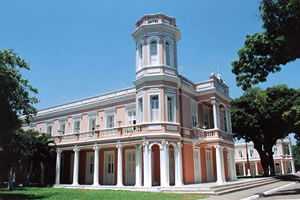
\includegraphics[width=16cm]{figuras/exemplo-1}
		}{
			\Fonte{\citeonline{UFC2012}.}
		}	
	\end{figure}
	
    Texto1 texto texto texto texto texto texto texto texto texto texto texto texto texto texto texto texto texto texto texto texto texto texto texto texto texto texto texto texto texto texto texto texto texto texto texto texto texto texto texto texto texto texto texto texto1.

    Texto2 texto texto texto texto texto texto texto texto texto texto texto texto texto texto texto texto texto texto. Texto texto texto texto texto texto texto texto texto texto texto texto texto texto texto texto texto texto texto2.

    Texto3 texto texto texto texto texto texto texto texto texto texto texto texto texto texto texto texto texto texto. Texto texto texto texto texto texto texto texto texto texto texto texto texto texto texto texto texto texto texto3.

    Texto4 texto texto texto texto texto texto texto texto texto texto texto texto texto texto texto texto texto texto. Texto texto texto texto texto texto texto texto texto texto texto texto texto texto texto texto texto texto texto4.

    A Figura \ref{fig:sondas} Texto texto texto texto texto texto texto texto texto texto texto texto texto texto texto texto texto texto texto. Texto texto texto texto texto texto texto texto texto texto texto texto texto texto texto texto texto texto texto3.

	\begin{figure}[h!]
		\centering
		\captionsetup{width=14cm}%Da mesma largura que a figura
		\Caption{\label{fig:sondas} Gráfico da Atmosfera Superior}	
		\UFCfig{}{
			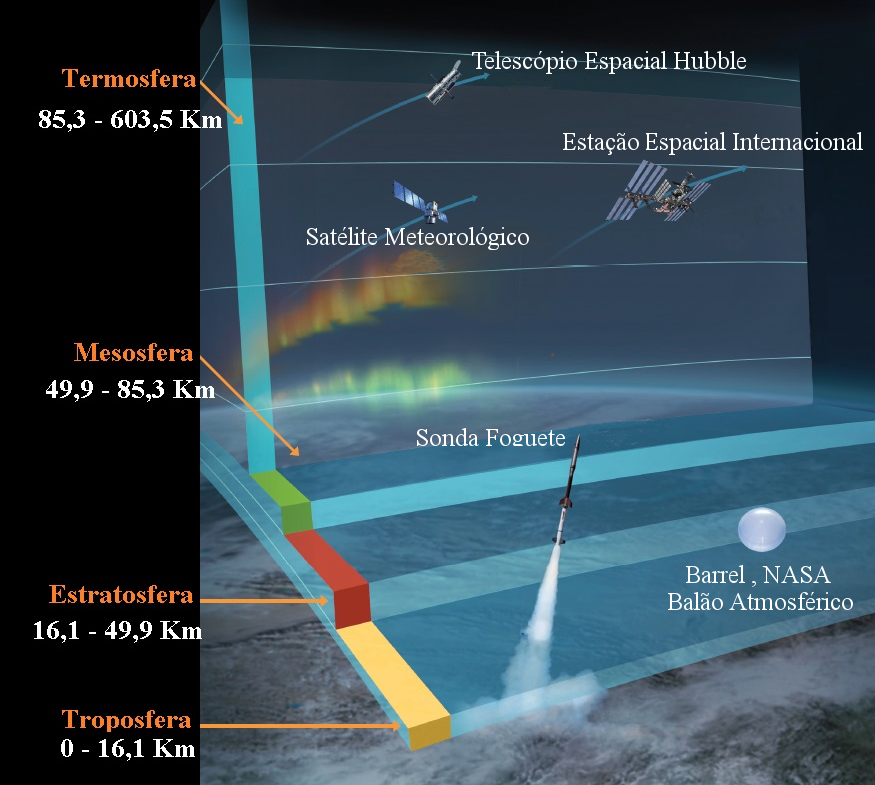
\includegraphics[width=14cm]{figuras/sondas}
		}{
			\Fonte{adaptado da \citeonline{NASA2016}.}}	
	\end{figure}

    Texto5 texto texto texto texto texto texto texto texto texto texto texto texto texto texto texto texto texto texto texto texto texto texto texto texto texto texto texto texto texto texto texto texto texto texto texto texto texto texto texto texto texto texto texto texto5.

    Texto6 texto texto texto texto texto texto texto texto texto texto texto texto texto texto texto texto texto texto texto texto texto texto texto texto texto texto texto texto texto texto texto texto texto texto texto texto texto texto texto texto texto texto texto texto5.

    Texto7 texto texto texto texto texto texto texto texto texto texto texto texto texto texto texto texto texto texto texto texto texto texto texto texto texto texto texto texto texto texto texto texto texto texto texto texto texto texto texto texto texto texto texto texto texto texto texto texto texto texto texto texto texto texto texto texto texto texto texto texto texto texto texto6.

    Evite terminar seções, capítulos e etc com figura. Procure escrever mais.

\section{Inserindo tabelas}\label{sec:tabelas}
    
    A Tabela \ref{tab:exemplo-1}... texto texto texto texto texto texto texto texto texto texto texto texto texto texto texto texto texto texto texto. Texto texto texto texto texto texto texto texto texto texto texto texto texto texto texto texto texto texto texto.
	
	\begin{table}[!h]
	\captionsetup{width=7cm}%Deixe da mesma largura que a tabela
	\Caption{\label{tab:exemplo-1} Um Exemplo de tabela alinhada que pode ser longa ou curta}%
	\IBGEtab{}{%
		\begin{tabular}{ccc}
			\toprule
			Nome & Nascimento & Documento \\
			\midrule \midrule
			Maria da Silva & 11/11/1111 & 111.111.111-11 \\
			Maria da Silva & 11/11/1111 & 111.111.111-11 \\
			Maria da Silva & 11/11/1111 & 111.111.111-11 \\
			\bottomrule
		\end{tabular}%
	}{%
	\Fonte{o autor.}%
	\Nota{esta é uma nota, que diz que os dados são baseados na
		regressão linear.}%
	\Nota[Anotações]{uma anotação adicional, seguida de várias outras.}%
    }
    \end{table}

	%\begin{table}[h!]	
	%	\centering
	%	\Caption{\label{tab:exemplo-1} Exemplo de tabela}	
	%	\UFCtab{}{
	%		\begin{tabular}{cll}
	%			\toprule
	%			Ranking & Exon Coverage & Splice Site Support \\
	%			\midrule \midrule
	%			E1 & Complete coverage by a single transcript & Both splice sites\\
	%			E2 & Complete coverage by more than a single transcript & Both splice sites\\
	%			E3 & Partial coverage & Both splice sites\\
	%			E4 & Partial coverage & One splice site\\
	%			E5 & Complete or partial coverage & No splice sites\\
	%			E6 & No coverage & No splice sites\\
	%			\bottomrule
	%		\end{tabular}
	%	}{
	%	\Fonte{elaborado pelo autor.}
	%}
	%\end{table}

\subsection{Exemplo de subseção} \label{sec:ex_sec}
	
    Texto texto texto texto texto texto texto texto texto texto texto texto texto texto texto texto texto texto texto texto texto texto texto texto texto texto texto texto texto texto texto texto texto texto texto texto texto texto texto texto texto texto texto texto texto.

    %acrlong{DATASUS},\acrlong{DNV},\acrlong{DO},\acrlong{ESF},\acrlong{IBGE},\acrlong{MFC},\acrlong{MI},\acrlong{MS},\acrlong{NV},\acrlong{ODM},\acrlong{OI},\acrlong{OMS},\acrlong{ONU},\acrlong{PNI},\acrlong{PSF},\acrlong{RIPSA},\acrlong{RN},\acrlong{SIM},\acrlong{SINASC},\acrlong{SUS},\acrlong{TMI},\acrlong{TMMFC}


    \begin{alineascomponto}
	    \item Integer non lacinia magna. Aenean tempor lorem tellus, non sodales nisl commodo ut
	    \item Proin mattis placerat risus sit amet laoreet. Praesent sapien arcu, maximus ac fringilla efficitur, vulputate faucibus sem. Donec aliquet velit eros, sit amet elementum dolor pharetra eget
	    \item Integer eget mattis libero. Praesent ex velit, pulvinar at massa vel, fermentum dictum mauris. Ut feugiat accumsan augue, et ultrices ipsum euismod vitae
	    \begin{subalineascomponto}
		    \item Integer non lacinia magna. Aenean tempor lorem tellus, non sodales nisl commodo ut
		    \item Proin mattis placerat risus sit amet laoreet.
	    \end{subalineascomponto}
    \end{alineascomponto}

\subsection{Uso de siglas} \label{sec:siglas}

    Para utilizar siglas, primeiro defina a sigla no arquivo "lista-de-abreviaturas-e-siglas"~ dentro da pasta "1-pre-textuais" com o comando 
    \begin{verbatim}
        \newacronym{ABNT}{ABNT}{Associação Brasileira de Normas Técnicas}
    \end{verbatim}
    Depois chame a sigla com o comando:
    \begin{verbatim}
        \gls{ABNT}
    \end{verbatim}
    Fica assim: \gls{ABNT}. A primeira vez que o comando é usado para uma determinada sigla, aparece o significado por extenso da sigla com a sua abreviação em seguida. A partir da segunda vez que o comando para uma determinada sigla é usado, aparace apenas a sigla. Por exemplo: \gls{ABNT}.  
    
    Veja o código fonte de outros exemplos: Teste de siglas \gls{TEST}, outros exemplos de siglas: \gls{DA}, \gls{MCEG}. 
    Repare que sempre as siglas estão sendo definidas primeiramente no arquivo ``lista-de-abreviaturas-e-siglas''.
\fi
	\chapter{Projeto do datalogger}
\label{chap:metodologia}

% \section{Motivação}

% A escolha entre uma dessas soluções, deve levar em conta o tipo de aplicação e o nível de criticidade dos dados levantados. Para levantamento de dados de temperatura de salas de armazenamento de vacinas, ou da umidade relativa do ar em uma cultura agrícola e afins, a escolha de um \textit{Datalogger} se mostra ideal. 



\section{Estudo de mercado}\label{sec:estudo_mercado}


% Um \textit{datalogger} é um dispositivo de funcionamento autônomo, que conta com sensores, memória interna e é capaz de realizar e disponibilizar a leitura de uma ou mais variáveis do ambiente e armazená-lo por um determinado período de tempo que pode ser de dias, meses ou até anos. 


Em busca de compreender propriedades como preço, dimensões e precisão de medição dos \textit{dataloggers} existentes no mercado atualmente, realizou-se um estudo no qual foi buscado quais dispositivos realizam a leitura de temperatura e umidade, possuem comunicação Wi-Fi ou Bluetooth e possuem uma opção de alimentação por bateria. Os dispositivos encontrados que atendem as especificações da pesquisa, que estão listados na tabela \ref{tab:dataloggers_novos}. 
	\begin{table}[!h]
	
	\captionsetup{width=7cm}%Deixe da mesma largura que a tabela
	\Caption{\label{tab:dataloggers_novos} \textit{Dataloggers: Preços e Mercados}}%
% 	\resizebox{\textwidth}{!}{
	\IBGEtab{}{%
		\begin{tabular}{ccccc}
			\toprule
			Modelo & Fabricante & Preço (R\$) & Mercado & Nível de Proteção \\
			\midrule \midrule
            RCW-360        & Elitech            &  1.499,00 & Nacional    & IP64/IP65 \\
            EL-WiFi-TH     & Lascar Electronics &  1.305,14 & Estrangeiro & IP55      \\
            TandD RTR-507B & TandD              &  2.242,57 & Estrangeiro & IP64      \\
            160 TH         & testo              &  2.842,00 & Nacional    & IP20
            \\
		    \bottomrule
		\end{tabular}%
	}{%
	\Fonte{o autor.}%
% 	\Nota{Todos os dispositivos medem temperatura e umidade relativa do ambiente}%
% 	\Nota[Legenda]{Na coluna de fabricantes, as letras representam os seguintes fabricantes\\
% 	A = Display Visions\\
% 	B = FLIR Extech\\
% 	C = Lascar Electronics\\
% 	D = O autor}%
    }
    % }
    \end{table}

Houve a necessidade de fazer essa busca no mercado no estrangeiro, dessa forma os preços apresentados dos itens que necessitam de importação levam em conta tanto o frete quanto as taxas alfandegárias de importação. Tendo em vista os valores de mercados encontrados, observa-se que é necessário que o hardware proposto deve possuir um preço unitário menor que R\$1.305,14. 


	\begin{table}[!h]
	
	\captionsetup{width=7cm}%Deixe da mesma largura que a tabela
	\Caption{\label{tab:dataloggers_novos_propriedades} \textit{Dataloggers: Propriedades}}%
	\resizebox{\linewidth}{!}{
	\IBGEtab{}{%
		\begin{tabular}{ccccccc}
			\toprule
			Modelo & Dimensões & Autonomia & Faixa de Leitura (ºC) & Precisão (ºC) & Umidade Relativa (\%) & Precisão(\%)\\
			\midrule \midrule
           RCW-360        & Não informado   & 3 meses       & -35 a 80 & 0,5 & 0 a 99 & 5    \\
           EL-WiFi-TH     & 82 x 70 x 23 mm & 6 meses       & -20 a 60 & 0,3 & 0 a 100 & 2    \\
           TandD RTR-507B & 62 x 47 x 19 mm & 10 meses      & -25 a 70 & 0,3 & 0 a 99  & 2,50 \\
           160 TH         & 76 x 64 x 22 mm & Não informado & -30 a 50 & 0,1 & 0 a 100 & 2   
            \\
	    \bottomrule
		\end{tabular}%
	}{%
	\Fonte{o autor.}%
% 	\Nota{Todos os dispositivos medem temperatura e umidade relativa do ambiente}%
% 	\Nota[Legenda]{Na coluna de fabricantes, as letras representam os seguintes fabricantes\\
% 	A = Display Visions\\
% 	B = FLIR Extech\\
% 	C = Lascar Electronics\\
% 	D = O autor}%
    }
    }
    \end{table}

A tabela \ref{tab:dataloggers_novos_propriedades} descreve quais algumas propriedades dos \textit{dataloggers} encontrados na busca, mas que são usadas como objetivo a ser alcançado no desenvolvimento do dispositivo proposto.


\section{Escopo de projeto}


% Definir o escopo do projeto foi o ponto de partida do desenvolvimento do dispositivo datalogger. Para isso, foi então definido que deveria ser desenvolvido um datalogger que fosse capaz de ler, persistir e disponibilizar os dados coletados à partir da leitura da temperatura, umidade relativa e luminosidade do ambiente em que ele esteja instalado. 

% A persistência dos dados coletados deve idealmente ser feita em uma mídia que removível que pudesse manter os dados armazenados por um longo período de tempo e que também seja capaz de suportar temperaturas um maiores que a temperatura ambiente. Além disso, os dados devem ser escritos de forma que seja facilitada a importação deles para ferramentas de visualização de dados. 

A ideia principal do projeto é desenvolver um datalogger de baixo custo de aquisição, dado suas características técnicas e deve ser um dispositivo capaz de ler temperatura, umidade relativa e luminosidade do ambiente em que ele estiver instalado. 

Essas leituras devem ser realizadas periodicamente de forma que o intervalo mínimo entre cada possa estar na casa dos segundos, se possível, e devem ser armazenadas em uma mídia de armazenamento de massa removível. Essa mídia deve manter os dados guardados por um período de tempo  de pelo menos 45 dias e suportar variações de temperaturas ligeiramente maiores ou menores que a temperatura média do local de instalação.

\section{Levantamento das especificações técnicas do hardware}

Realizando a análise do escopo definido, foram então levantadas as especificações que o hardware proposto deve atender. À partir dessas especificações será então criado uma arquitetura para o hardware, que elencará quais componentes, protocolos e afins deverão ser adotados.

    \begin{enumerate}
        \item Possuir a capacidade de ler a temperatura do ambiente;
        \item Possuir a capacidade de ler a umidade relativa do ambiente;
        \item Possuir a capacidade de ler o nível de luminosidade do ambiente;
        \item Possuir alternativa de alimentação direta ou via bateria;
        \item Leitura de sensores via interfaces \gls{I2C}, \gls{SPI} e/ou \gls{UART};
        \item Formatação dos dados lidos dos sensores para auxiliar no envio e/ou coleta;
        \item Persistir os dados em um cartão SD para a coleta manual dos dados;
        \item Persistência dos dados coletados por no mínimo 45 dias;
        % \item Interface de comunicação via rádio LoRa;
        % \item Envio periódico dos dados guardados via LoRaWan;
        \item Possuir interface de interação com o usuário;
        \item Permitir a configuração da taxa de amostragem das variáveis lidas;
        % \item Permitir o envio de dados coletados via interface de comunicação sem fio;
        % \item Permitir o recebimento e aplicação de configurações via interface de comunicação sem fio;
        % \item (Ideia pra placa: Deixar uma interface pra gravação do firwmare)
        % \item Possuir proteção contra intempéries;
        % \item Preferencialmente escolher componentes com propriedades de operação da classe automotiva; 
        % \item Alertas para quando algum dado lido extrapolar um valor pré-configurado;
        % \item Possuir um display lcd ou oled pra ajudar na interação com o usuário;
        % \item Ser possível expandir a quantidade de sensores facilmente e de forma plug\&play;
        % \item Possuir possibilidade de atualização de firwmare over-the-air;
        % \item Possuir células fotovoltaicas para recarregas a bateria;
        % \item Possuir circuito de recarregamento das baterias;

    \end{enumerate}

\section{Definição da arquitetura de hardware}

Tendo sido levantados as especificações do projeto, esses são analisados a fim de se criar uma arquitetura de hardware do projeto. Fazem parte dessa arquitetura o diagrama de blocos do hardware proposto, que irá nortear a definição de que quais componentes que serão necessários para a construção do dispositivo. 

Junto ao levantamento dos componentes, também são elencado quais propriedades eles deverão possuir para que as especificações do projeto sejam atendidos. Uma vez que isso seja feito, é então dado início a seleção desses componentes no mercado de componentes eletrônicos de acordo com o especificado na etapa anterior de levantamento de componentes.

\subsection{Diagrama de blocos}

No diagrama de blocos do dispositivo datalogger proposto, cada bloco é um objeto que representa um componente que deve fazer parte da do hardware. Além disso, são também elencados as interfaces de comunicação, se necessário, que cada objeto deverá ter com outros objetos. 

Analisando as especificações técnicas são definidos quais objetos deverão compor  o hardware. Alguns desses objetos podem ser compostos de objetos menores, dependendo do nível de complexidade que eles apresentam. Assim, o seguintes objetos são definidos:

 \begin{itemize}
     \item Unidade de processamento;
     \item Sensor de luminosidade;
     \item Sensor de temperatura; 
     \item Sensor de umidade;
     \item Unidade de alimentação;
     \item Unidade de interface de usuário;
    %  \item Unidade de interface de comunicação USB;
     \item Unidade de leitura e escrita de dados em cartão SD;
 \end{itemize}

À partir da definição dos objetos, é então elaborado o diagrama de blocos do dispositivo a ser desenvolvido. O diagrama deste projeto segue abaixo.

    \begin{figure}[h!]
            \captionsetup{width=16cm}
    		\Caption{\label{fig:datalogger_blocks} Diagrama de Blocos do datalogger}
    		%\centering
    		\UFCfig{}{
    			\fbox{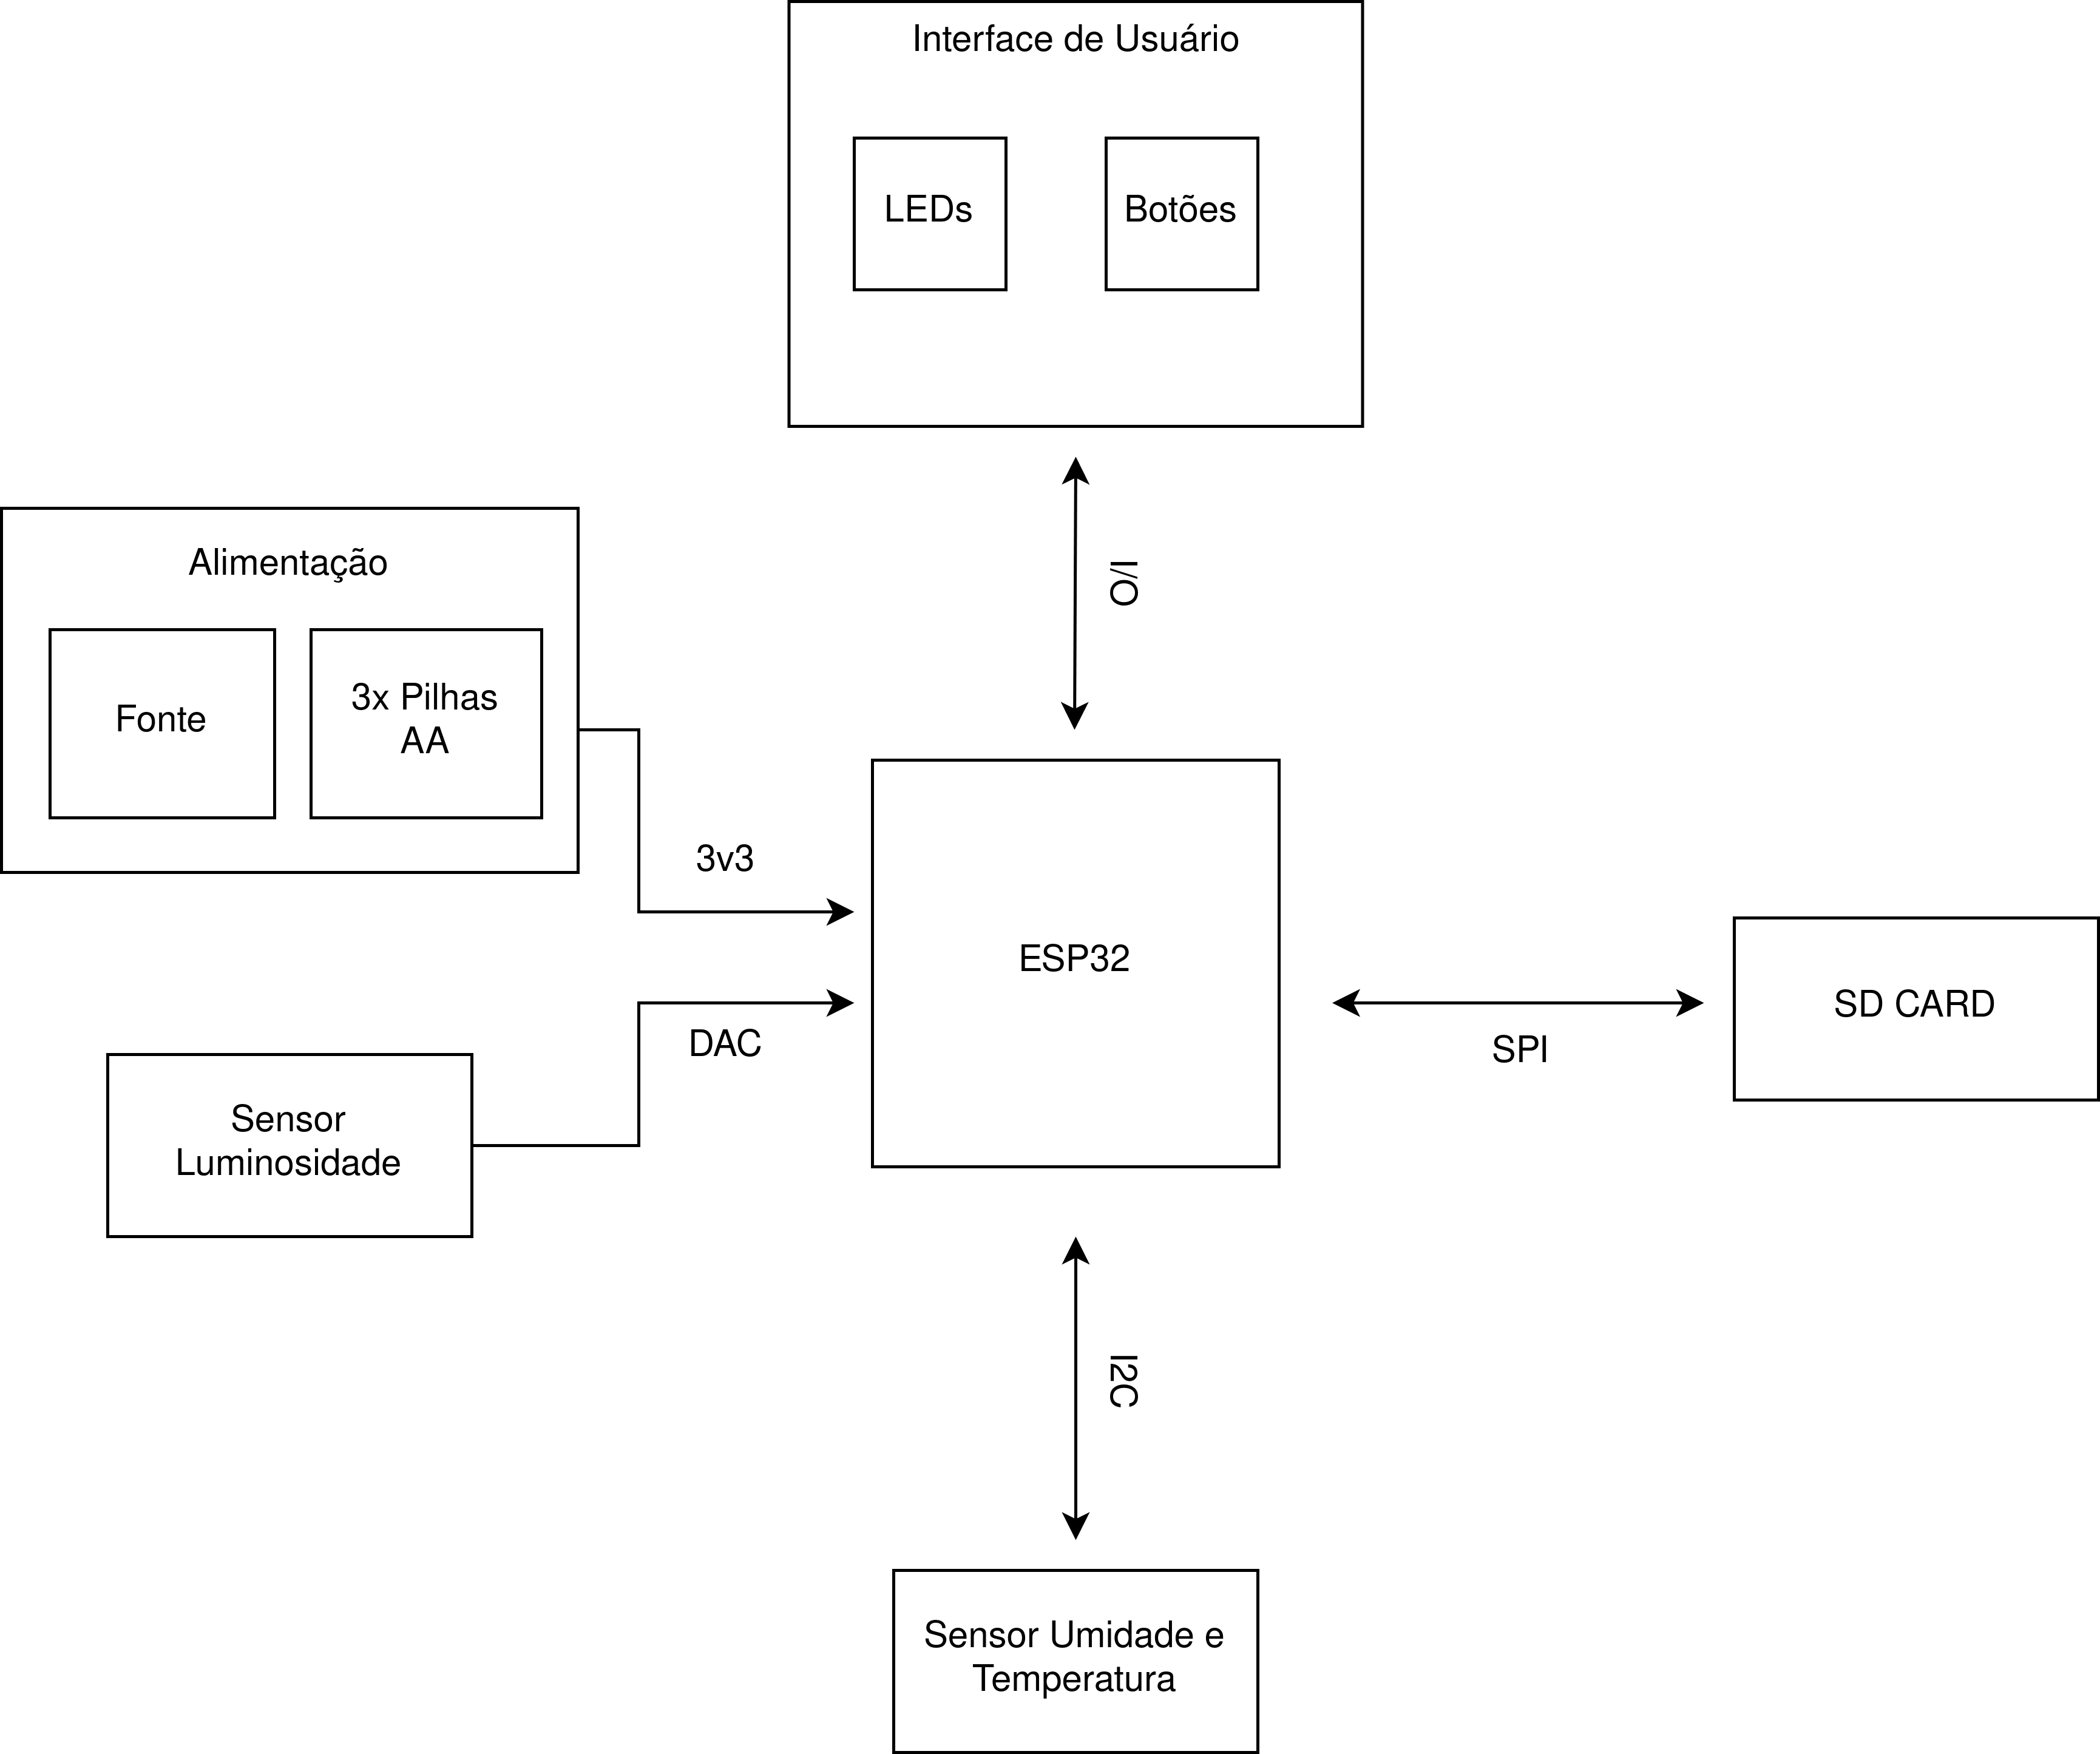
\includegraphics[width=\textwidth]{figuras/capitulo3/datalogger_tcc.drawio.png}}
    		}{
    			\Fonte{elaborado pelo autor (2022).}
    		}	
   \end{figure}

\subsection{Levantamento de tipos de componentes}\label{subsec:levantamento_tipos}


Uma vez que se tenha o diagrama de blocos criado, é dado início ao processo de seleção de componentes. Nesta etapa são analisados as especificações técnicas e o diagrama de blocos do projeto a fim de se levantar quais componentes e quais propriedades esses componentes devem possuir para serem considerados ideais para o desenvolvimento do hardware. 

Assim, para cada objeto do diagrama foram levantado quais tipos de componentes fazem parte da definição desse objeto, com o objetivo de orientar a procura e escolha dos componentes eletrônicos nos distribuidores. Os tipos de componentes levantados seguem abaixo: 

\begin{itemize}
 
 \item Unidade de processamento
     \begin{itemize}
         \item Microcontrolador que opere em 3V3 e possua interfaces de comunicação \gls{I2C}, \gls{SPI} e \gls{UART};
     \end{itemize}

 \item Sensores de umidade, temperatura e luminosidade; 
  \begin{itemize}
     \item Sensor de umidade relativa e temperatura que opere em 3V3;
     \item Sensor de luminosidade que opere em 3V3;
 \end{itemize}
 
 \item Unidade de alimentação:
     \begin{itemize}
         \item Suporte para baterias do tipo AA;
         \item Circuito que forneça 3,3 V de tensão de alimentação ao hardware;
    \end{itemize} 

\item Unidade de interface de usuário: 

    \begin{itemize}
        \item LEDs multicoloridos;
        \item Botões tácteis.
    \end{itemize}
%  \item Unidade de interface de comunicação USB;
%     \begin{itemize}
%         \item Conector de comunicação USB.
%     \end{itemize}
 
 \item Unidade de leitura e escrita de dados em cartão SD;
     \begin{itemize}
         \item Suporte de leitura de cartão microSD;
     \end{itemize}
 %Acho que aqui é melhor fazer uma análise dos requisitos e ir comentando qual componente atende aos requisitos X e Y.
\end{itemize}

\subsection{Recomendações para seleção de componentes}\label{subsec:recomendacoes_componentes}

Tendo sido levantado quais os tipos de componentes devem fazer parte da construção do hardware proposto, é preciso dar início ao processo escolha dos componentes no mercado de componentes eletrônicos. Contudo, algumas recomendações devem ser feitas antes que essa fase do projeto seja iniciada a fim de se evitar custos adicionais seja durante a fase de desenvolvimento, seja na fase de produção do hardware desenvolvido. 

Assim, como primeira recomendação pode ser destacado a escolha de componentes ativos como microcontroladores, \gls{ASIC}s ou semelhantes, que estejam com produção ativa e que tenham um tempo de vida útil garantida pela fabricante de pelo menos 10 anos à partir da data em que projeto inicia sua fase de produção. Essa recomendação visa garantir a longevidade do dispositivo desenvolvido, visto que quando há a descontinuidade de produção ou falta desse tipo de componente no mercado, isso gera um custo extra ao fabricante que se desejar manter seu hardware sendo produzido vai ou precisar adquirir e manter um estoque próprio desses componentes, ou arcar com os custos extras de retrabalho do seu hardware para substituir o componente que está em falta por um equivalente. 

Já para componentes passivos, como resistores, capacitores e afins, é preciso um cuidado semelhante uma vez que também há problema de descontinuidade da produção para esse tipo de componente pelos seus fabricantes. Contudo o processo de substituição por um componente equivalente é mais simples uma vez que um componente com as mesmas propriedades do escolhido inicialmente podem ser produzidos por mais de um fabricante. 

Dessa forma, visando aproveitar essa característica dos componentes passivos é recomendado que no momento da seleção desses componentes sejam escolhidos os que possuam propriedades comuns de serem encontradas no mercado de componentes eletrônicos. Por exemplo, no caso da seleção de um capacitor eletrolítico de montagem em superfície, é recomendado que as principais propriedades, capacitância, dimensões físicas e tensão de operação sejam comuns de serem encontradas no mercado. Do contrário, se um capacitor possuir dimensões físicas que somente alguns fabricantes produzem, isso pode levar a um custo extra na produção de um hardware, devido a necessidade se realizar um retrabalho nele para que um capacitor com dimensões diferentes do componente inicialmente utilizado possa ser adotado como substituto. 

%   Os componentes ativos (CIs e afins) devem estar em produção ativa e possuir um fim de vida no mercado de pelo menos 10 anos no futuro à partir da data de escolha deles;
\subsection{Seleção de componentes eletrônicos}

Nessa etapa do projeto são buscados em distribuidores de componentes eletrônicos os que melhor se encaixam nas especificações técnicas do hardware proposto, assim, para cada um dos tipos de componentes levantados na subseção \ref{subsec:levantamento_tipos} essa busca será realizada. 

% Contudo, devido a grande quantidade desses distribuidores no mercado de componentes eletrônicos, a busca desses componentes foi restringida a somente alguns desses distribuidores que são elencados abaixo:

% \begin{itemize}
%     \item Arrow Electronics 	
%     \item Arrow.cn 	
%     \item Avnet 	
%     \item Digi-Key 	
%     \item Element14 	
%     \item Farnell 	
%     \item Future Electronics 	
%     \item LCSC 	
%     \item Mouser 	
%     \item Newark
% \end{itemize}

\subsubsection{Microcontrolador}\label{subsubsec:esp32_modulo}


Para a escolha desse componente em um primeiro momento foram analisadas as especificações do projeto e levantadas algumas características que o microcontrolador ideal para o hardware proposto deveria possuir. A primeira dessas características é a presença dos periféricos \gls{UART}, \gls{SPI} e \gls{I2C} no componente escolhido devido a necessidade de comunicação com os sensores ou a mídia removível usando um desses protocolos.

Foi observado também a necessidade do microcontrolador ter um baixo consumo energético durante sua operação, de forma que seja possível manter o dispositivo funcionando ininterruptamente por 45 dias com uma alimentação provinda de um conjunto de pilhas. Por conta disso no momento da seleção, além dessa característica, foi buscado um microcontrolador que possuísse também um modo de operação em hibernação, no qual o microcontrolador mantém energizado somente seus periféricos essenciais para diminuir o consumo energético ao máximo. 

Tendo sido feitas essas considerações, foi então escolhido o módulo microcontrolador da Espressif Systems, ESP32-S3-WROOM-1-N8, que é formado pela associação do \gls{SOC} ESP32-S3 com uma memória \textit{Flash} \gls{SPI}. Algumas das propriedades desse módulo são:

    \begin{itemize}
        \item Quantidade de portas de Entradas/Saída: 36;
        \item Periféricos: CAN, I2C, SPI, USART e USB;
        \item Tipo e tamanho da memória de programa: Flash SPI de 8MB;
        \item Interfaces de comunicação: Wi-Fi 802.11 b/g/n, Bluetooth LE Radio.
        \item Tamanho da memória de dados: 512kB;
        \item Tensão de operação: 3V a 3,6V;
        \item Faixa de temperatura de operação: -40ºC a 85ºC;
    \end{itemize}
    
    
    \begin{figure}[h!]
            \captionsetup{width=16cm}
    		\Caption{\label{fig:datalogger_blocks} Diagrama de Blocos do \gls{SOC} ESP32-S3}
    		%\centering
    		\UFCfig{}{
    			\fbox{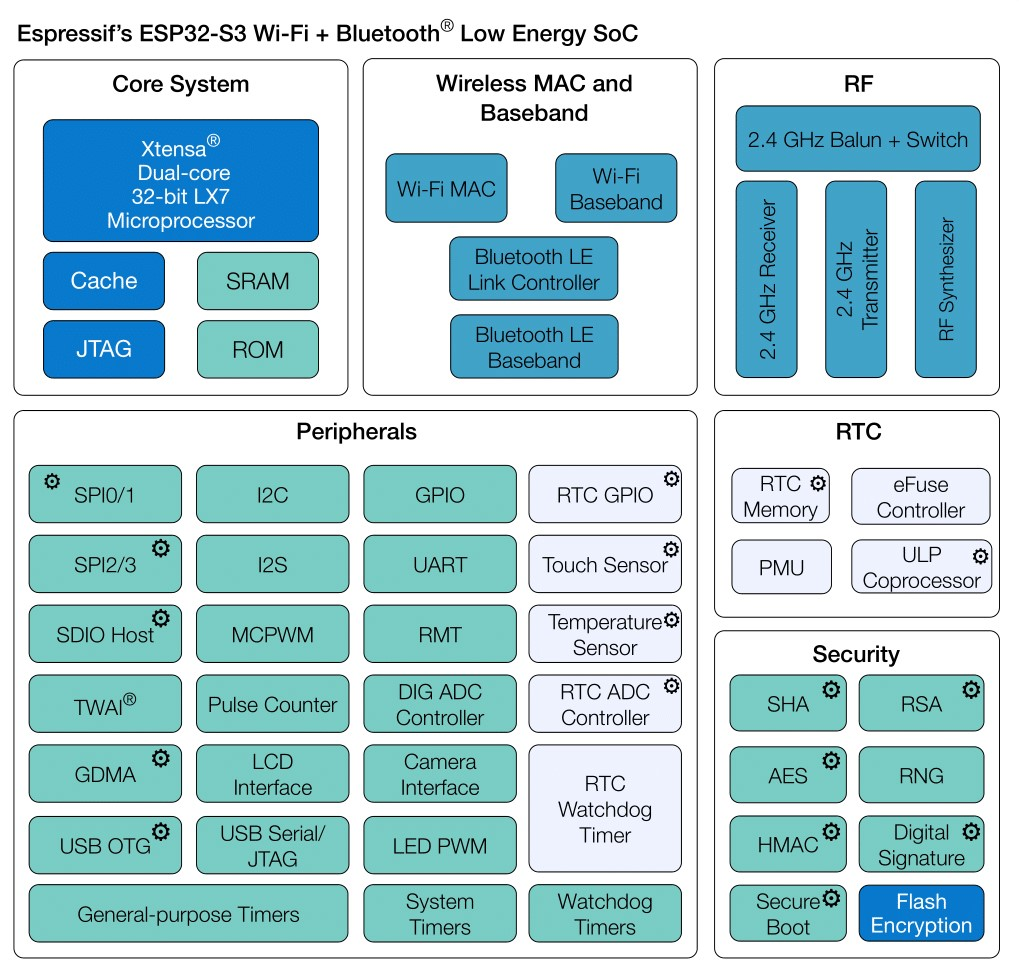
\includegraphics[width=\textwidth]{figuras/capitulo3/esp32-s3_datasheet_en-02.jpg}}
    		}{
    			\Fonte{Espressif Systems (2022).}
    		}	
   \end{figure}    
    
    
    
    

Juntamente com essas propriedades, outros fatores que influenciaram na escolha desse módulo foram seu preço unitário de US\$ 3,29 e uma garantia de 12 anos de longevidade garantida pela Espressif Systems à partir do dia primeiro de janeiro de 2021. 

\subsubsection{Sensor de umidade e temperatura}

Para realizar a leitura da umidade relativa do ambiente foi escolhido o sensor da Texas Instruments HDC1080, que possui também um sensor de temperatura integrado. Esse sensor é capaz de operar em uma faixa de tensão que vai de 2,7 V a 5,5 V, possui uma interface I²C e um modo de operação em hibernação no qual o consumo de corrente elétrica é reduzido a 100 nA.

Além dessas propriedades, esse sensor possui também uma acurácia média de 2\% para leitura da umidade relativa do ambiente, e uma acurácia de 0,2\% na média para a leitura da temperatura do ambiente. Essas características o tornam ideal para o hardware proposto.

\subsubsection{Sensor de luminosidade}

Foi adotado para leitura do nível de luminosidade de um ambiente, o sensor LDR (do inglês Light Dependent Resistor - resistor dependente de luz) devido sua simplicidade de operação e baixo custo. Seu uso pede somente a associação com um resistor para formação de um circuito divisor de tensão, e que o microcontrolador utilizado possua um conversor analógico-digital em uma de suas portas. 





\subsubsection{Componentes das interface de usuário, comunicação USB e cartão SD}

De acordo com o levantado na seção \ref{subsec:levantamento_tipos}, os componentes da interface de usuário devem ser LEDs, botões tácteis e um alarme sonoro. Por serem componentes mais genéricos, não houve necessidade de se escolher fabricante ou modelo específico para cada um deles. Houve apenas as seguintes restrições: 

\begin{itemize}
    \item LEDs e o alarme sonoro devem possuir tensão de operação de 3,3 V;
    \item Os botões tácteis e LEDs devem ser de montagem do tipo PTH enquanto o alarme sonoro deve preferencialmente ser de montagem em superfície.
\end{itemize}

Já para as interfaces de comunicação USB e leitura do cartão microSD, são necessários um conector do tipo micro USB e um suporte de leitura para cartão microSD, respectivamente. Também não há restrição de fabricante ou modelo para esses componentes uma vez que são componentes genéricos. 


\subsubsection{Fonte de alimentação}\label{subsubsec:fonte_alimentacao}

Para o correto funcionamento de todos os demais componentes do hardware proposto, uma tensão de operação de 3,3 V é necessária. Contudo, conforme especificado na seção \ref{subsec:levantamento_tipos}, o hardware deve possuir suporte para alimentação fornecida por fonte externa ou proveniente de baterias do tipo AA. Esse tipo de bateria fornece até 1,5 V para cada unidade, de forma que para alimentar o hardware proposto é necessário um conjunto dessas pilhas AA associadas em série.

Devido essa possibilidade de uso de duas fontes de alimentação, podem ocorrer casos em que essas duas fontes estejam ligadas ao hardware ao mesmo tempo fazendo com que a fonte convencional passe a alimentar as pilhas e vice-versa. Assim, pra evitar essa interação, foi necessário desenvolver um circuito que fizesse a escolha entre a fonte convencional ou as pilhas para alimentar o hardware. 

Foi escolhido um transistor \gls{MOSFET} de canal P em associação com um resistor de 10 k$\Omega$ para realizar esse seleção. A tensão fornecida pela fonte externa é ligada ao terminal \textit{gate} do transistor enquanto a tensão proveniente das pilhas é ligado ao seu terminal \textit{source}. Dessa forma, quando não há tensão vinda de fonte convencional o transistor entra em sua região de saturação, permitindo que haja um fluxo de corrente do \textit{source} ao \textit{drain}, terminal esse que é conectado ao ponto de entrada de alimentação do hardware, no qual também é conectado a fonte externa. 

É nesse ponto de entrada que é comum as duas fontes de alimentação que ocorre a interação entre elas, podendo gerar algum dano ao hardware e/ou as pilhas caso essas não sejam recarregáveis. Para complementar esse circuito de seleção, foi necessário um diodo com seu ânodo conectado ao terminal \textit{drain} do transistor e seu cátodo conectado a esse ponto comum de alimentação, para impedir que haja fluxo de corrente da fonte externa às pilhas. 

Contudo, para a seleção do diodo que seria utilizado nesse circuito, foi necessário notar que a queda de tensão de 0,70 V causada pelos diodos comuns afetaria a tensão total fornecida pelas pilhas e prejudicaria a autonomia do hardware. Dessa forma foi dado preferência a escolha de um diodo do tipo schottky, que causa uma queda de tensão entre 0,15 V e 0,45 V o que impacta positivamente na autonomia final do hardware quando utilizando pilhas. Para atender essa necessidade foi escolhido o diodo schottky ON Semiconductor NSR0320MW2T1, que causa uma queda de tensão máxima de 0,45 V.

Para conclusão do circuito de alimentação e visando definir um longo tempo de autonomia para o hardware proposto, foi definido que devem ser utilizadas quatro pilhas do tipo AA em série, o que totaliza uma tensão de alimentação de 6 V, sendo necessário assim a necessidade de utilização de um regulador de tensão que regule esse valor para 3,3 V. Foi escolhido então o regulador de tensão \textit{low-dropout} (LDO em inglês) Diodes Incorporated AP2114HA-3.3TRG1 para realizar essa tarefa. Esse regulador suporta até 6,5 V como entrada e fornece uma tensão fixa de 3,3 V e uma corrente de até 1 A, mas apresentando uma queda de até 450 mV quando a tensão de entrada se aproxima da tensão de saída. 

Como esse regulador receberá como entrada a tensão do ponto de alimentação comum as duas fontes, esse valor se soma a ao valor queda de tensão causada pelo diodo schottky do sub-circuito de seleção das fontes, causando uma queda total de até 0,9 V na tensão fornecida pelas pilhas AA, impondo assim a 4,2 V o mínimo que as pilhas devem fornecer para um pleno funcionamento do hardware. 


Por fim as características do circuito de alimentação do hardware podem ser resumidas como segue:

\begin{itemize}
    \item Tensão máxima de entrada: 6,5 V;
    \item Tensão mínima de entrada: 4,2 V;
    \item Quantidade de pilhas AA necessárias: 4;
    \item Tensão típica de saída: 3,3 V;
    \item Corrente Máxima de saída: 1 A;
\end{itemize}


% uma vez que para atingir sua tensão de alimentação ideal seria necessário utilizar pelo menos três pilhas, que juntas em série fornecem 4,5 V mas devido essa queda de tensão só forneceriam 3,8 V

% seriam necessários de três a quatro pilhas

% Assim, foi escolhido o diodo  

% porque a queda de tensão causada por ele é menor do que a queda causada por um diodo comum é de 0,70 V contra os 0,45 V do diodo schottky. 

% Essa diferença se mostra importante porque, além dessa queda de tensão, há também a queda de tensão inerente ao regulador, que pode ser de até 0,450 V, totalizando uma queda de até 0,750 V na alimentação via pilhas. 




% A escolha desse tipo de diodo em detrimento ao diodo comum se deu porque a queda de tensão nesse é de 0,7 V, enquanto nesse diodo schottky a queda é de aproximadamente 0,3 V. 

% Essa queda precisa ser suplantada quando houver somente o uso das pilhas como fonte de alimentação e como cada uma é capaz de entregar até 1,5 V, um conjunto de quatro pilhas AA, totalizando 6V, é o necessário para alimentar corretamente o hardware proposto. 













% \begin{itemize}
%     \item Módulo Microcontrolador: De acordo com sua folha de dados, o módulo microcontrolador consome pelo menos 50mA de corrente para sua operação. Uma vez que o hardware proposto não irá fazer utilização dos rádios Wi-Fi ou Bluetooth disponíveis no módulo, a corrente máxima consumida será de 90mA.
    
%     \item Sensor de temperatura e umidade: Também de acordo a folha de dados desse componente o consumo médio de corrente é de apenas 1,3 $\mu$A para leituras constantes, com um pico de 7,2 mA mas somente quando a função de auto aquecimento é acionada. Contudo, caso nenhuma leitura esteja sendo feita, o sensor consome apenas 100 nA.
    
%     \item Cartão microSD: Para leitura e escrita de dados em cartão microSD é consumido em média 100 mA de corrente para cada operação, podendo ocorrer picos de 200mA. 
    
%     \item Componentes da interface de usuário: 
%     \begin{itemize}
%         \item LEDs: Para o uso dos LEDs da interface de usuário, o consumo de corrente médio é de 20mA para cada LED utilizado, podendo chegar a 50 mA quando em pico.
%         \item Alarme sonoro: A média de consumo de corrente desse componente é de 5 mA, com picos de 8 mA.
%         \item Botões tácteis: O consumo máximo desse componente é de 50 mA; 
%     \end{itemize}
    
% \end{itemize}



% À partir desses valores, foi então levantado o consumo em casos nos quais todos os componentes estão sendo utilizados ao mesmo tempo. Assim, quando da situação em que todos os componentes estão sendo utilizados e operando com pico de consumo, obtém-se um total de 405 mA de consumo. Já para o caso em que todos os componentes estejam sendo utilizados mas dentro da faixa de consumo médio de cada um, o consumo médio total é de 225 mA. 

% Para atender a especificação de funcionamento por meio de baterias, foi definido que um conjunto de pilhas AA se adequaria melhor devido não só a facilidade como também do baixo valor unitário de aquisição. 




% conjunto de quatro pilhas AA atenderia a esse requisito, tendo em vista que cada pilha fornece 1,5 V de tensão a associação de quatro pilhas em série é capaz de fornecer um total de 6 V de tensão.  


% À partir dessas informações, foi definido que um conjunto de quatro pilhas AA, no qual cada uma fornece 1,5 V de tensão, obtendo-se assim uma fonte de 6 V de tensão. Além disso, uma bateria desse tipo é capaz de fornecer até


% Dessa forma, para que a especificação de alimentação por pilhas por no mínimo 45 dias seja atendida e sabendo-se que cada pilha pode fornecer 1,5 V de tensão, é necessário a associação em série de quatro pilhas.


% Cada pilha é capaz de fornecer 1,5 V 





% Como essa tensão de alimentação por baterias está acima da especificação de 3,3 V para todo o hardware, é necessário um circuito que diminua essa tensão. Foi então escolhido o regulador linear de tensão AP2114HA-3.3TRG1 para que a tensão de 6 V fosse diminuída até a tensão de 3,3 V, para o correto funcionamento dos demais componentes. 






\section{Desenvolvimento do hardware}

\subsection{Esquemático Eletrônico}

\subsubsection{Circuito de alimentação}

Primeiro circuito a ser criado, foram seguidas as recomendações e adotados os componentes indicados na Seção \ref{subsubsec:fonte_alimentacao} para a construção desse circuito. Além desses componentes, foi adicionado também ao circuitos alguns componentes necessários ao regulador segundo sua folha de dados.


    \begin{figure}[h!]
            \captionsetup{width=10cm}
    		\Caption{\label{fig:datalogger_blocks} Esquemático Circuito de Alimentação Parte 1}
    		%\centering
    		\UFCfig{}{
    			\fbox{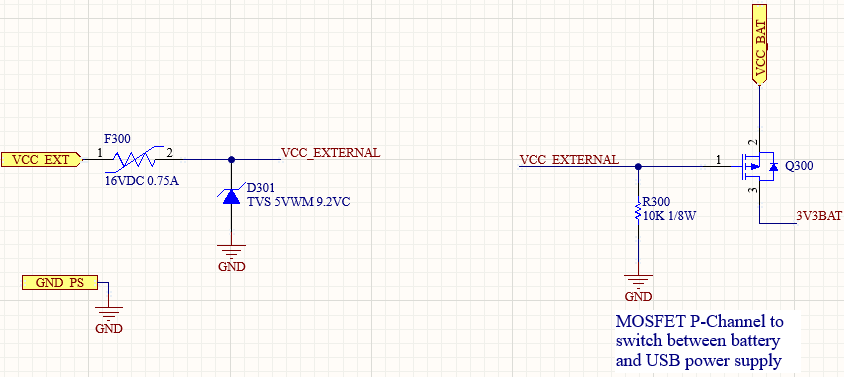
\includegraphics[width=0.9\textwidth]{figuras/capitulo3/esquematicos/power_1.png}}
    		}{
    			\Fonte{elaborado pelo autor (2022).}
    		}	
   \end{figure}    

    \begin{figure}[h!]
        \captionsetup{width=10cm}
		\Caption{\label{fig:datalogger_blocks} Esquemático Circuito de Alimentação Parte 2}
		%\centering
		\UFCfig{}{
			\fbox{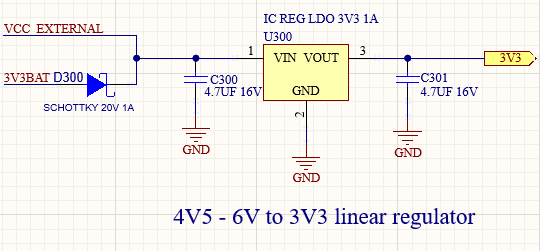
\includegraphics[width=0.9\textwidth]{figuras/capitulo3/esquematicos/power_2.png}}
		}{
			\Fonte{elaborado pelo autor (2022).}
		}	
\end{figure}    
\newpage

% Como o hardware pode ser alimentado tanto por um conjunto de pilhas quanto por uma fonte de alimentação convencional, pode ocorrer casos em que essas duas fontes estejam ligadas ao hardware ao mesmo tempo fazendo com que a fonte convencional tente alimentar as pilhas e vice-versa. Assim, pra evitar essa interação, foi necessário desenvolver um circuito que fizesse a escolha entre a fonte convencional ou as pilhas para alimentar o hardware. 

% Para isso, foi utilizado um transistor MOSFET de canal P em associação com um resistor de 10 k$\Omega$ para realizar esse seleção. A tensão fornecida pela fonte convencional é ligada ao terminal \textit{gate} do transistor enquanto a tensão proveniente das pilhas é ligado ao seu terminal \textit{source}. Dessa forma, quando não há tesão vinda de fonte convencional o transistor entra em sua região de saturação, permitindo que haja um fluxo de corrente do \textit{source} ao \textit{drain}, terminal esse que será conectado ao regulador de tensão do circuito de alimentação. 

% Contudo como o regulador possui uma única entrada e o hardware possui duas fontes de alimentação possíveis, foi necessário utilizar o diodo schottky ON Semiconductor NSR0320MW2T1G na ligação entre o terminal \textit{drain} do transistor chaveador e o ponto de entrada de tensão do regulador, para evitar que a corrente vinda da fonte externa se encaminhasse para o terminal \textit{drain} do transistor. 

% A escolha desse tipo de diodo em detrimento ao diodo comum se deu porque a queda de tensão nesse é de 0,7 V, enquanto nesse diodo schottky a queda é de aproximadamente 0,3 V. Essa diferença se mostra importante porque, além dessa queda de tensão, há também a queda de tensão inerente ao regulador, que pode ser de até 0,450 V, totalizando uma queda de até 0,750 V na alimentação via pilhas. 

% Essa queda precisa ser suplantada quando houver somente o uso das pilhas como fonte de alimentação e como cada uma é capaz de entregar até 1,5 V, um conjunto de quatro pilhas AA, totalizando 6V, é o necessário para alimentar corretamente o hardware proposto. 

\subsubsection{Sensores LDR e HDC1080}

O sensor LDR pede somente um circuito formado pela sua associação em série com um resistor de 10 k$\Omega$, para a formação um circuito divisor de tensão, o qual será conectado a um dos conversores analógico-digital do módulo microcontrolador.


    \begin{figure}[h!]
            \captionsetup{width=7cm}
    		\Caption{\label{fig:datalogger_blocks} Esquemático sensor LDR}
    		%\centering
    		\UFCfig{}{
    			\fbox{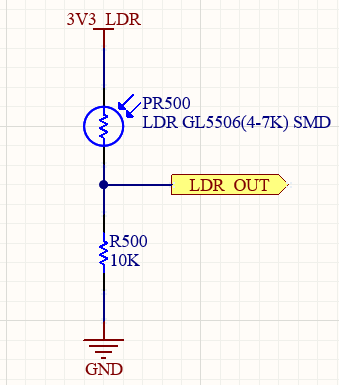
\includegraphics[width=0.4\textwidth]{figuras/capitulo3/esquematicos/light_sensor.png}}
    		}{
    			\Fonte{elaborado pelo autor (2022).}
    		}	
   \end{figure}  

\newpage


O sensor de temperatura e umidade HDC1080 por fazer sua comunicação com o módulo microcontrolador utilizando o protocolo \gls{I2C}, necessitou de resistores \textit{pull-up} de 10 k$\Omega$ conectados em paralelo a cada uma de suas linhas de dados, de acordo com as recomendações da fabricante.

    \begin{figure}[h!]
            \captionsetup{width=7cm}
    		\Caption{\label{fig:datalogger_blocks} Esquemático sensor HDC1080}
    		%\centering
    		\UFCfig{}{
    			\fbox{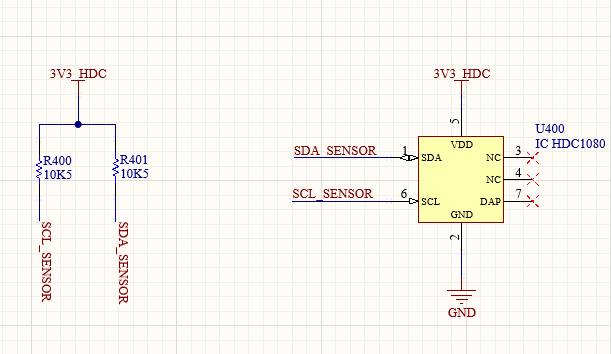
\includegraphics[width=0.8\textwidth]{figuras/capitulo3/esquematicos/temp_sensor.png}}
    		}{
    			\Fonte{elaborado pelo autor (2022).}
    		}	
   \end{figure}  




\subsubsection{Cartão microSD}

Para o circuito de comunicação com o cartão microSD foi necessário conectar cada uma de suas linhas de dados a resistores \textit{pull-up} de 10 k$\Omega$ de acordo com recomendações da fabricante do módulo microcontrolador, a fim de se evitar que essas linhas assumam um estado indefinido. 

Devido ao grande consumo de corrente, 100 mA em média mas podendo ter picos de 200 mA, foi necessário adicionar um transistor MOSFET de baixo quesciente na linha de alimentação do cartão microSD para que, quando não estiver sendo utilizado para gravação ou leitura de dados, permaneça desligado e não haja desperdício de energia.

    \begin{figure}[h!]
            \captionsetup{width=7cm}
    		\Caption{\label{fig:datalogger_blocks} Esquemático suporte microSD}
    		%\centering
    		\UFCfig{}{
    			\fbox{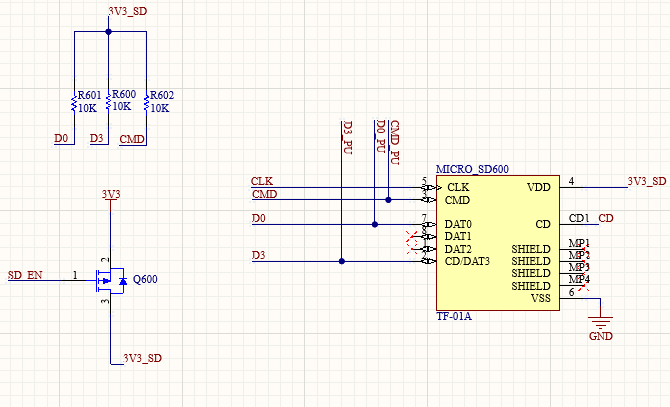
\includegraphics[width=\textwidth]{figuras/capitulo3/esquematicos/sdcard.png}}
    		}{
    			\Fonte{elaborado pelo autor (2022).}
    		}	
   \end{figure}  



\subsubsection{Circuito de controle}


O circuito de controle compreende o módulo microcontrolador e os circuitos auxiliares necessários para seu funcionamento. Em seu pino de alimentação foi necessário a associação em paralelo de dois capacitores, de 22$\mu$F e 100nF, seguindo recomendações da sua folha de dados, para garantir o mínimo de perturbação em sua linha de alimentação. 

Para permitir a reinicialização do dispositivo quando preciso, foi também externado o pino três do módulo que tem como função habilitar o seu funcionamento quando ligado ao terra. Assim, foi seguido a recomendação da fabricante de usar um botão táctil em associação com capacitores para formar o circuito de habilitação de funcionamento do módulo microcontrolador.

Também foi externado o pino 27 do módulo que quando ligado ao terra, indica que o dispositivo deverá inicializar em modo \textit{download}, no qual será possível realizar a gravação de um novo \textit{firmware}. Do contrário, o módulo será inicializado no modo \gls{SPI} em busca de conjunto de instruções para executar. 

    \begin{figure}[h!]
            \captionsetup{width=10cm}
    		\Caption{\label{fig:datalogger_blocks} Esquemático circuito de controle}
    		%\centering
    		\UFCfig{}{
    			\fbox{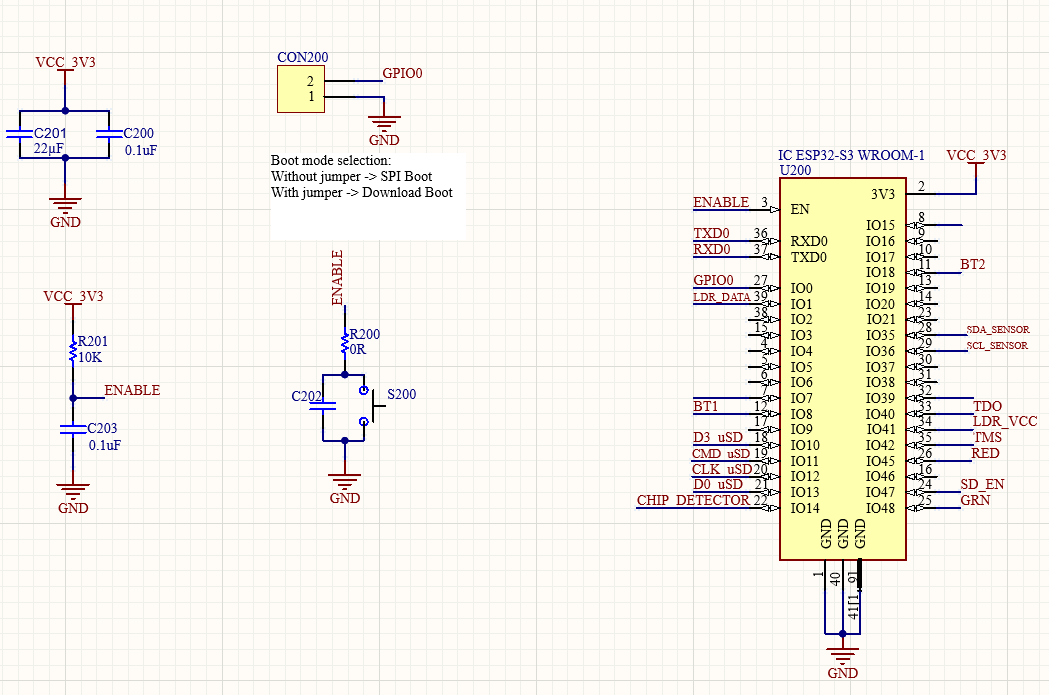
\includegraphics[width=\textwidth]{figuras/capitulo3/esquematicos/controller.png}}
    		}{
    			\Fonte{elaborado pelo autor (2022).}
    		}	
   \end{figure}  





\subsection{Design PCI}




Após terem sido criados os esquemáticos eletrônicos do hardware projetado, foi então passado para a fase de desenvolvimento do leiaute a \gls{PCI} do hardware proposto. Como passo inicial, foram primeiramente definidos alguns requisitos que a placa deveria atender para manter baixo seu custo de produção:

\begin{itemize}
    \item A placa deve possuir preferencialmente a largura de 50 centímetros e comprimento de 50 centímetros;
    
    \item A placa deverá ser projetada em duas camadas somente; 
\end{itemize}


\subsubsection{\textit{Stackup} da PCI}

O \textit{stackup} de uma PCI define as características e parâmetros que o conjunto de cobre e materiais dielétricos que uma placa projetada deve possuir. Assim, como as especificações do projeto pedem, é feito o \textit{stackup} para de uma placa de circuito impresso com duas camadas.

É definido FR-4 como material dielétrico de base para a produção dessa placa, devido não só sua popularidade, como também pela sua característica de retardar fogo em caso de incêndio, e sua espessura deve ser de 1,6 mm (63 mils). Já a o cobre aplicado sobre o dielétrico possui uma espessura 0,036 mm (1,4 mils), o que equivale a aproximadamente a quantidade de 1 oz/pé², e uma impedância típica de 50$\Omega$. A placa produzida tem uma espessura total de 1.6 mm.


    \begin{figure}[h!]
            \captionsetup{width=7cm}
    		\Caption{\label{fig:pcb_stackup} \textit{Stackup} da PCI}
    		%\centering
    		\UFCfig{}{
    			\fbox{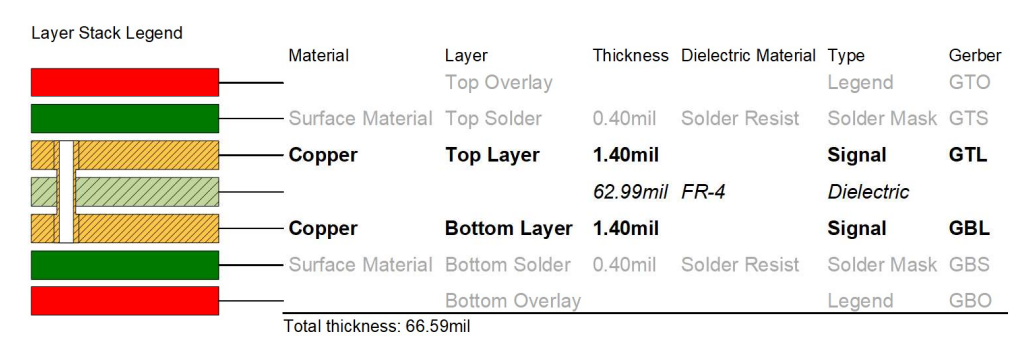
\includegraphics[width=\textwidth]{figuras/capitulo3/pcb/pcb_stackup.png}}
    		}{
    			\Fonte{elaborado pelo autor (2022).}
    		}	
   \end{figure}  


\subsubsection{Particionamento e posicionamento}

Como primeiro passo foi realizado um particionamento funcional do espaço definido para a placa como uma forma de não só organizar os componentes que pertencem a um mesmo circuito em determinados grupos, como também posicionar esses grupos no espaço da placa de maneira a auxiliar no roteamento dos desses circuitos posteriormente. Assim, foi elaborado o seguinte particionamento:


    \begin{figure}[h!]
            \captionsetup{width=16cm}
    		\Caption{\label{fig:datalogger_blocks} Particionamento funcional da placa}
    		%\centering
    		\UFCfig{}{
    			\fbox{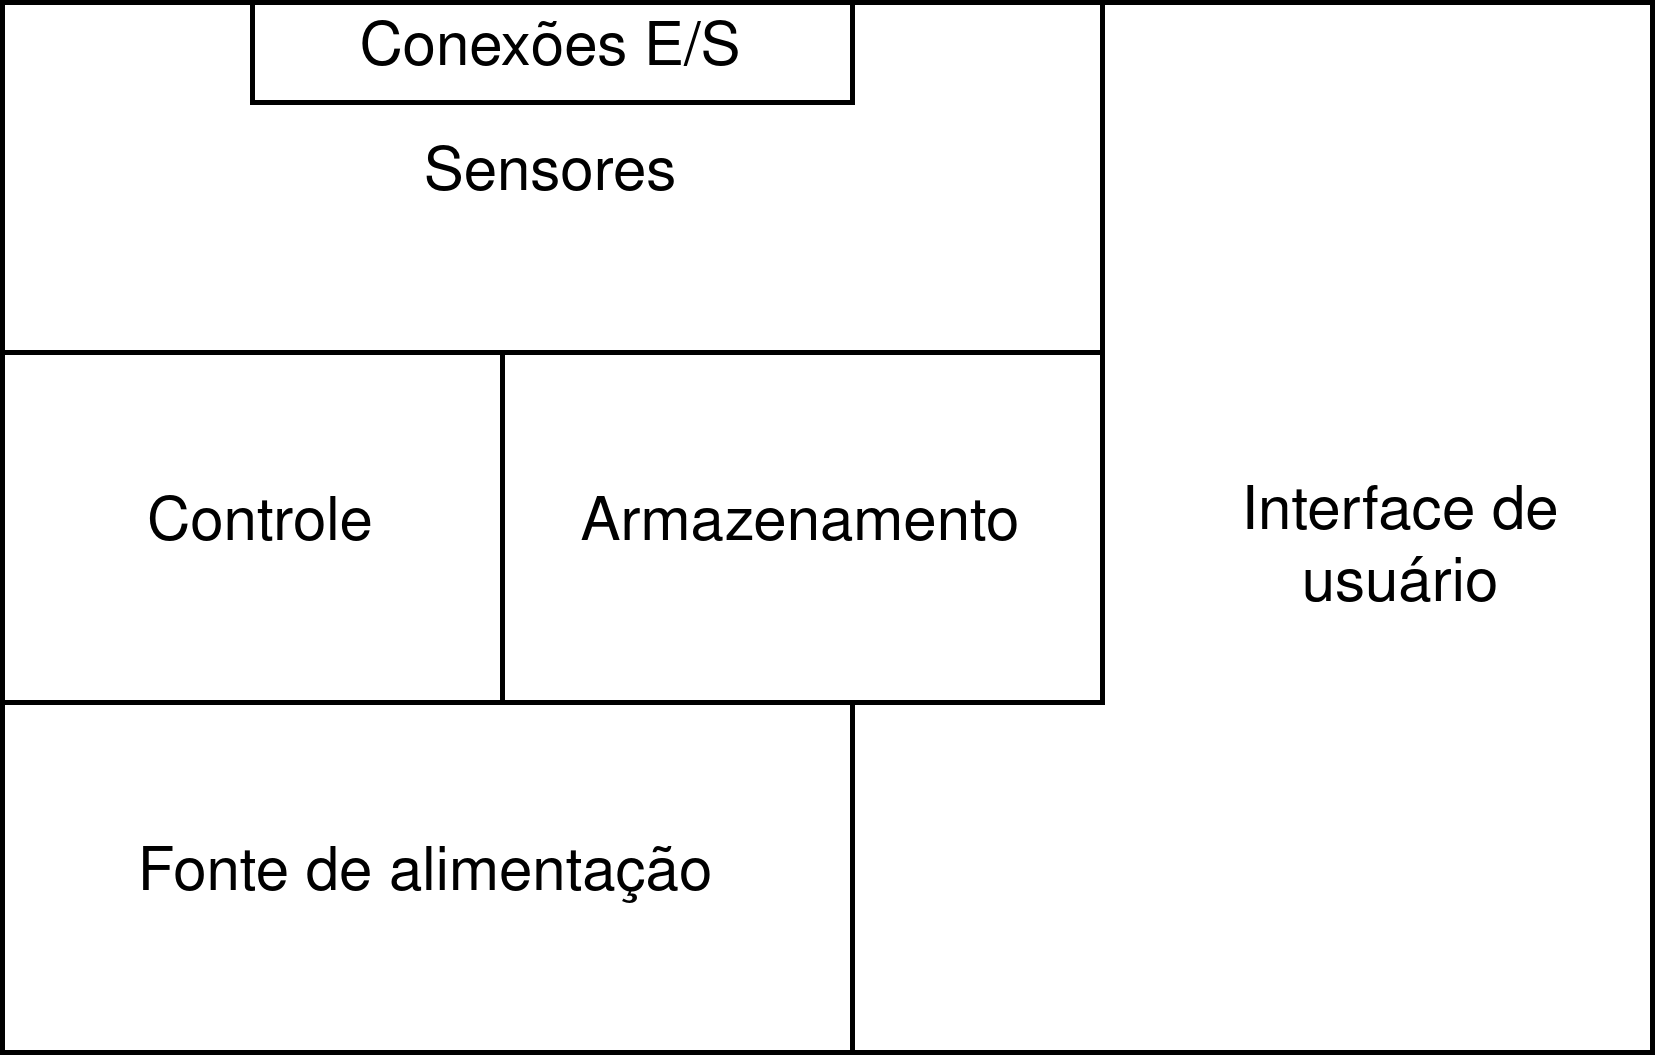
\includegraphics[width=\textwidth]{figuras/capitulo3/particionamento.drawio.png}}
    		}{
    			\Fonte{elaborado pelo autor (2022).}
    		}	
   \end{figure}


Em seguida foram trazidos os desenhos dos componentes descritos nos esquemáticos eletrônicos para a visão de projeto PCB e dado início ao processo de organização dos componentes no espaço definido para a placa, com o circuito de controle sendo o primeiro a ser colocado e organizado nesse espaço.

Foi procurado posicionar o módulo microcontrolador no espaço que lhe foi reservado no particionamento, porém devido sua antena de comunicação Wi-Fi, foi seguida a recomendação da fabricante e o módulo foi posicionado de forma que a antena ficasse além das bordas da placa. Em seguida foram adicionados dois capacitores em paralelo com valores recomendados pela fabricante, paralelos a linha de alimentação do módulo para atuarem como um circuito de desacoplamento. Os demais componentes desse circuito que compõem o sub-circuito de habilitação de operação do módulo microcontrolador, foram posicionados também o mais próximo possível do módulo com exceção ao botão táctil e seus componentes auxiliares, que foram colocados na borda oposta da placa.

Em seguida, os componentes do circuito da fonte de alimentação do hardware foram colocados e posicionados de tal forma que O regulador de tensão U300 juntamente com seus componentes auxiliares foram posicionados próximos a linha de tensão do módulo microcontrolador a fim de atenuar interferências em sua alimentação. Os conectores desse circuito, juntamente com os componentes do sub-circuito foram posicionados próximos a borda da placa a fim de facilitar a conexão dos cabos de alimentação, mas também próximos o suficiente do regulador de tensão para evitar interferências em sua linha de alimentação. 

Os circuitos dos sensores foram colocados também na área que lhes foi reservada, com os sensores estando o mais próximo possíveis do módulo microcontrolador. Contudo, para os circuitos da interface de usuário e do leitor de cartão microSD não foi possível ajustar seus componentes de forma que fosse colocados exatamente nos espaços reservados no particionamento devido a sobreposição de algumas ligações desses circuitos.

Assim, o leitor de cartão microSD foi posicionado ao centro da placa de forma que ficasse oposto ao posicionamento do módulo microcontrolador. Para que fosse facilitado seu roteamento, o leitor foi colocado na face inferior da placa. Já os componentes do circuito de interface de usuário foram colocados o mais próximo das pontas das placa possível, de forma que também ficassem na mesma face mas do lado oposto ao módulo microcontrolador.

    \begin{figure}[h!]
            \captionsetup{width=10cm}
    		\Caption{\label{fig:pcb_placement} Posicionamento final dos componentes}
    		%\centering
    		\UFCfig{}{
    			\fbox{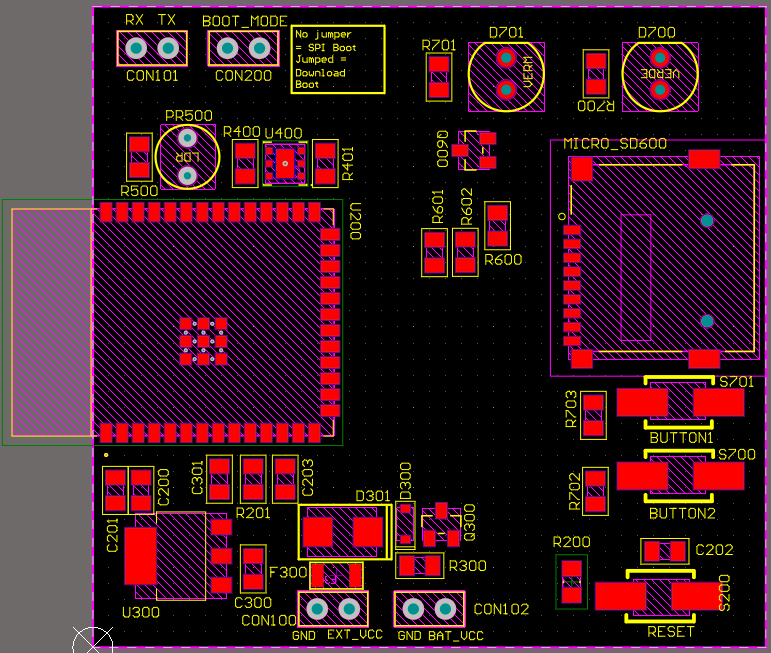
\includegraphics[width=0.8\textwidth]{figuras/capitulo3/pcb/pcb_no_route.png}}
    		}{
    			\Fonte{elaborado pelo autor (2022).}
    		}	
   \end{figure}

\newpage


\subsubsection{Roteamento}

O processo de roteamento foi realizado utilizando-se inicialmente regras genéricas para tamanho de trilhas sendo configuradas para possuírem 10 mil de largura. As primeiras trilhas a serem roteadas foram as de conexões de comunicação e leitura de sensores devido sua importância em relação às demais conexões, assim pode-se ter maior liberdade de espaço para realizar o roteamento. Na sequência foi realizado o roteamento dos componentes do circuito da interface de usuário, que foram tomados por último para esse processo devido suas conexões possuírem uma baixa complexidade. 


    \begin{figure}[h!]
            \captionsetup{width=10cm}
    		\Caption{\label{fig:pcb_placement} Roteamento de sinais}
    		%\centering
    		\UFCfig{}{
    			\fbox{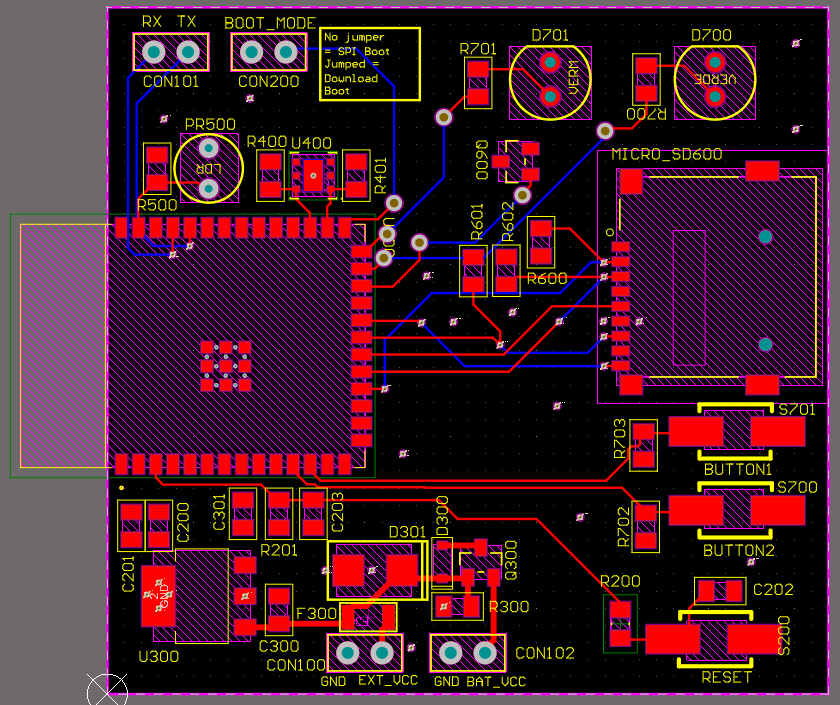
\includegraphics[width=0.7\textwidth]{figuras/capitulo3/pcb/pcb_signlas_route.png}}
    		}{
    			\Fonte{elaborado pelo autor (2022).}
    		}	
   \end{figure}



Após esses circuitos, faz-se o roteamento do circuito de alimentação com o processo sendo iniciado pelas conexões dos sub-circuitos de entrada de alimentação e de seleção da fonte de alimentação. Tendo sido feitas as conexões de todos os componentes desse circuito, foi então dado início ao processo de conectar os demais circuitos da placa à alimentação.

Procurou-se fazer que houvesse uma trilha de alimentação que alcançasse maioria dos componentes realizando um contorno no sentido anti-horário ao redor do centro da placa. Foi escolhido essa estratégia em detrimento da criação de múltiplas trilhas de alimentação saindo de um ponto comum, para evitar a criação de vários pequenos ciclos de corrente ao longo da placa, o que poderia gerar interferências eletromagnéticas não só entre os circuitos do hardware mas também com o ambiente externo. 
    
    \begin{figure}[h!]
            \captionsetup{width=10cm}
    		\Caption{\label{fig:pcb_placement} Roteamento de sinais e alimentação}
    		%\centering
    		\UFCfig{}{
    			\fbox{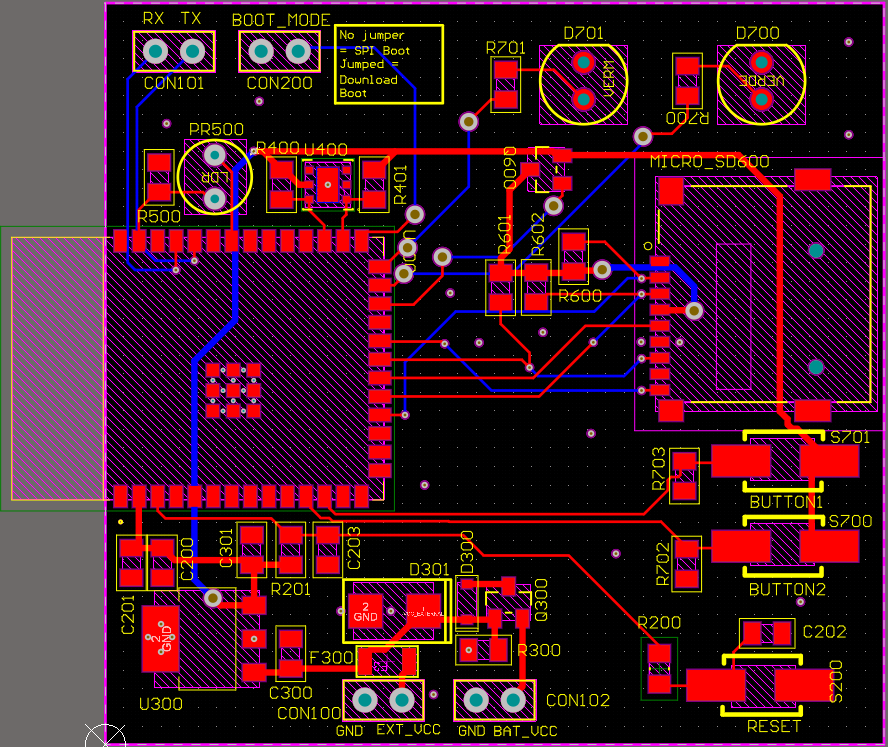
\includegraphics[width=0.7\textwidth]{figuras/capitulo3/pcb/pcb_with_power.png}}
    		}{
    			\Fonte{elaborado pelo autor (2022).}
    		}	
   \end{figure}


% \newpage

Por fim é feito a criação de planos de terra de forma que toda a placa, em ambas as faces, fique coberta por esses planos. Isso torna possível interligar todos os componentes ao terra de forma que esse ponto de ligação está o mais próximo possível do componente, o que evita que o caminho de retorno da corrente seja muito longo e acabe gerando interferências eletromagnéticas.

    \begin{figure}[h!]
            \captionsetup{width=10cm}
    		\Caption{\label{fig:pcb_power_top} Plano de terra face superior}
    		%\centering
    		\UFCfig{}{
    			\fbox{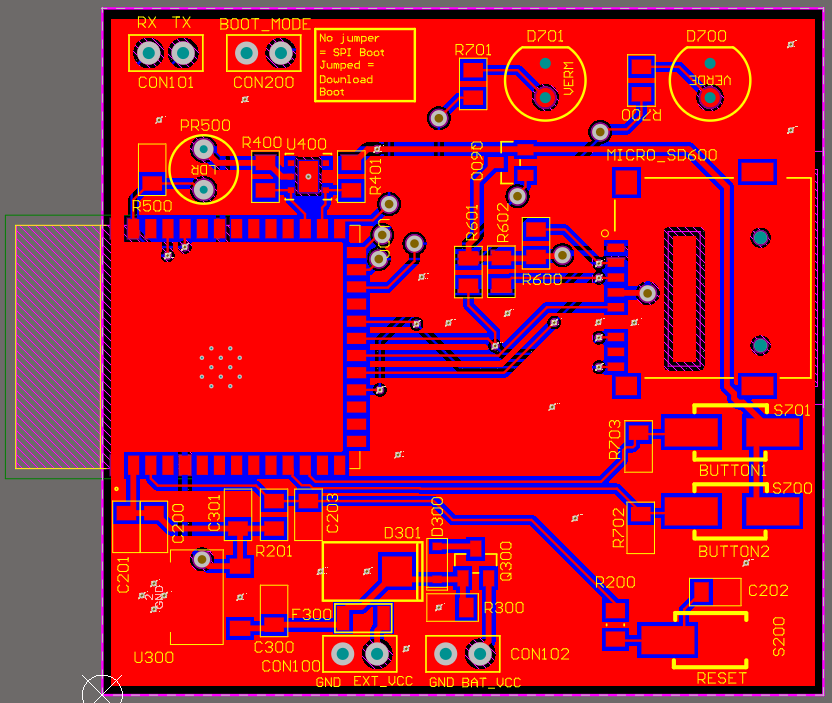
\includegraphics[width=0.7\textwidth]{figuras/capitulo3/pcb/pcb_top_plane.png}}
    		}{
    			\Fonte{elaborado pelo autor (2022).}
    		}	
   \end{figure}

    \begin{figure}[h!]
            \captionsetup{width=10cm}
    		\Caption{\label{fig:pcb_power_bottom} Plano de terra face inferior}
    		%\centering
    		\UFCfig{}{
    			\fbox{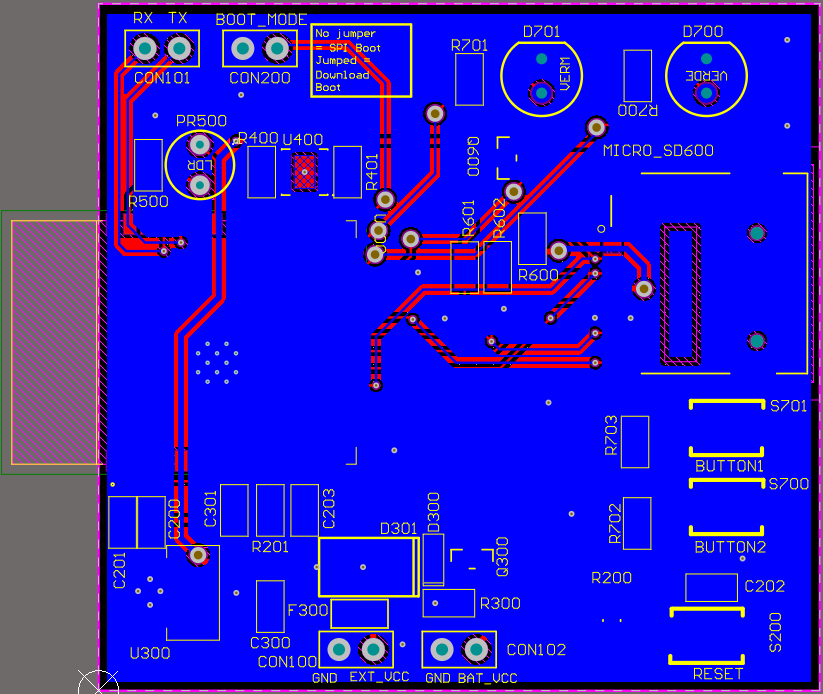
\includegraphics[width=0.7\textwidth]{figuras/capitulo3/pcb/pcb_bottom_plane.png}}
    		}{
    			\Fonte{elaborado pelo autor (2022).}
    		}	
   \end{figure}












% \section{Definição da arquitetura de software}



% \subsection{Diagrama de blocos do software}


% \subsubsection{Diagrama organizacional de software}





\iffalse
-------------------------------------------------------------------------------------------------

% Texto texto texto texto texto texto texto texto texto texto texto texto texto texto texto texto texto texto texto texto texto texto texto texto texto texto texto texto texto texto texto texto texto texto texto texto texto texto texto texto texto texto texto texto texto texto texto texto texto texto texto texto texto texto texto texto texto texto texto texto texto texto texto texto texto texto texto texto texto.

% Texto texto texto texto texto texto texto texto texto texto texto texto texto texto texto texto texto texto texto texto texto texto texto texto texto texto texto texto texto texto texto texto texto texto texto texto texto texto texto texto texto texto texto texto texto texto texto texto texto texto texto texto texto texto texto texto texto texto texto texto texto texto texto texto texto texto texto texto texto.

\section{Exemplo de alíneas}\label{sec:exemplo-de-algoritmos-e-figuras}

    Texto texto texto texto texto texto texto texto texto texto texto texto texto texto texto texto texto texto texto texto texto texto texto texto texto texto texto texto texto texto texto texto texto texto texto texto texto texto texto texto texto texto texto texto texto texto texto texto texto texto texto texto texto texto texto texto texto texto texto texto texto texto texto texto texto texto texto texto texto.

    %\begin{algorithm}[h!]
    %	\SetSpacedAlgorithm
    %	\caption{\label{exemplo-de-algoritmo}Como escrever algoritmos no \LaTeX2e}
    %	\Entrada{o proprio texto}
    %	\Saida{como escrever algoritmos com  Latex:}% \LaTeX2e }
    %	\Inicio{
    %		inicialização;
    %		\Repita{fim do texto}{
    %			leia o atual;
    %			\Se{entendeu}{
    %				vá para o proximo\;
    %				próximo se torna o atual;}
    %			\Senao{volte ao início da seção;}
    %		}
    %	}	
    %\end{algorithm}

    Texto texto texto texto texto texto texto texto texto texto texto.

    %\begin{algorithm}[H]
    %	\Entrada{o proprio texto}
    %	\Saida{como escrever algoritmos com \LaTeX2e }
    %	\Inicio{
    %		inicialização\;
    %		\Repita{fim do texto}{
    %			leia o atual\;
    %			\Se{entendeu}{
    %				vá para o próximo\;
    %				próximo se torna o atual\;}
    %			\Senao{volte ao início da seção\;}
    %		}
    %	}
    %	\caption{Exemplo de Algoritmo Versao 02}
    %\end{algorithm}

    %\begin{algorithm}
    %	\begin{algorithmic}
    %	\Entrada{o proprio texto}
    %	\Saida{como escrever algoritmos com \LaTeX2e }	
    %	\end{algorithmic}
    %\end{algorithm}

    Exemplo de alíneas com números:

    \begin{alineascomnumero}
	    \item Texto texto texto texto texto texto texto texto texto texto texto texto .
	    \item Texto texto texto texto texto texto texto texto texto texto texto texto .
	    \item Texto texto texto texto texto texto texto texto texto texto texto texto .
	    \item Texto texto texto texto texto texto texto texto texto texto texto texto .
	    \item Texto texto texto texto texto texto texto texto texto texto texto texto .
	    \item Texto texto texto texto texto texto texto texto texto texto texto texto .
    \end{alineascomnumero}

    Texto texto texto texto texto texto texto texto texto texto texto texto texto texto texto texto texto texto texto texto texto texto texto texto texto texto texto texto texto texto texto texto texto texto texto texto texto texto texto texto texto texto texto texto texto texto texto texto texto texto texto texto texto texto texto texto texto texto texto texto texto texto texto texto texto texto texto texto texto.

    Ou então figuras podem ser incorporadas de arquivos externos, como é o caso da \autoref{fig-grafico-1}. Se a figura que ser incluída se tratar de um diagrama, um gráfico ou uma ilustração que você mesmo produza, priorize o uso de imagens vetoriais no formato PDF. Com isso, o tamanho do arquivo final do trabalho será menor, e as imagens terão uma apresentação melhor, principalmente quando impressas, uma vez que imagens vetorias são perfeitamente escaláveis para qualquer dimensão. Nesse caso, se for utilizar o Microsoft Excel para produzir gráficos, ou o Microsoft Word para produzir ilustrações, exporte-os como PDF e os incorpore ao documento conforme o exemplo abaixo. No entanto, para manter a coerência no uso de software livre (já que você está usando LaTeX e abnTeX),  teste a ferramenta InkScape\index{InkScape}. ao CorelDraw\index{CorelDraw} ou ao Adobe Illustrator\index{Adobe! Illustrator}.  De todo modo, caso não seja possível  utilizar arquivos de imagens como PDF, utilize qualquer outro formato, como JPEG, GIF, BMP, etc.  Nesse caso, você pode tentar aprimorar as imagens incorporadas com o software livre \index{Gimp}Gimp. Ele é uma alternativa livre ao Adobe Photoshop\index{Adobe! Photoshop}.

\section{Usando Fórmulas Matemáticas}

Para escrever um símbolo matemático no texto, escreva símbolo entre cifrões, por exemplo, $\alpha$, $\beta$ e $\gamma$ são símbolo do alfabeto grego. Se você quiser inserir equações enumeradas, siga a estrutura de
\begin{equation}
    \label{eq:indices}
	k_{n+1} = n^2 + k_n^2 - k_{n-1}.
\end{equation}
Observe a pontuação, pois a equação faz parte da frase e do parágrafo. Como a equação faz parte da frase, não se utiliza o \textit{label} numérico \ref{eq:indices}. 

Quando for citar a Equação \ref{eq:indices} novamente no texto, utiliza-se o \textit{label} numérico. Repare que a palavra ``Equação'' foi escrita com ``E'' maiúsculo. 

Um exemplo de equações com frações é dado por
\begin{equation}
	\label{eq:fracao}
		\begin{aligned}
			x = a_0 + \cfrac{1}{a_1
				+ \cfrac{1}{a_2
					+ \cfrac{1}{a_3 + \cfrac{1}{a_4} } } }.
		\end{aligned}
	\end{equation}

Texto texto texto texto texto texto texto texto texto texto texto texto texto texto texto texto texto texto texto texto texto texto texto texto texto texto texto texto texto texto texto texto texto texto texto texto texto texto texto texto texto texto texto texto texto texto texto texto texto texto texto texto texto texto texto texto texto texto texto texto texto texto texto texto texto texto texto texto texto
	\begin{equation}
		\begin{aligned}
			k_{n+1} = n^2 + k_n^2 - k_{n-1}.
		\end{aligned}
	\end{equation}
	
Texto texto texto texto texto texto texto texto texto texto texto texto texto texto texto texto texto texto texto texto texto texto texto texto texto texto texto texto texto texto texto texto texto texto texto texto texto texto texto texto texto texto texto texto texto texto texto texto texto texto texto texto texto texto texto texto texto texto texto texto texto texto texto texto texto texto texto texto texto
	\begin{equation}
	\label{eq:trigo}
		\begin{aligned}
			\cos (2\theta) = \cos^2 \theta - \sin^2 \theta
		\end{aligned}.
	\end{equation}
	
Texto texto texto texto texto texto texto texto texto texto texto texto texto texto texto texto texto texto texto texto texto texto texto texto texto texto texto texto texto texto texto texto texto texto texto texto texto texto texto texto texto texto texto texto texto texto texto texto texto texto texto texto texto texto texto texto texto texto texto texto texto texto texto texto texto texto texto texto texto
	\begin{equation}
	\label{eq:matriz}
		\begin{aligned}
			A_{m,n} =
			\begin{pmatrix}
			a_{1,1} & a_{1,2} & \cdots & a_{1,n} \\
			a_{2,1} & a_{2,2} & \cdots & a_{2,n} \\
			\vdots  & \vdots  & \ddots & \vdots  \\
			a_{m,1} & a_{m,2} & \cdots & a_{m,n}
			\end{pmatrix}
		\end{aligned}.
	\end{equation}

Texto texto texto texto texto texto texto texto texto texto texto texto texto texto texto texto texto texto texto texto texto texto texto texto texto texto texto texto texto texto texto texto texto texto texto texto texto texto texto texto texto texto texto texto texto texto texto texto texto texto texto texto texto texto texto texto texto texto texto texto texto texto texto texto texto texto texto texto texto
	\begin{equation}
	\label{eq:sistema}
		\begin{aligned}
			f(n) = \left\{ 
			\begin{array}{l l}
			n/2 & \quad \text{if $n$ is even}\\
			-(n+1)/2 & \quad \text{if $n$ is odd}
			\end{array} \right.
		\end{aligned}.
	\end{equation}
Texto texto texto texto texto texto texto texto texto texto texto texto texto texto texto texto texto texto texto texto texto texto texto texto texto texto texto texto texto texto texto texto texto texto texto texto texto texto texto texto texto texto texto texto texto texto texto texto texto texto texto texto texto texto texto texto texto texto texto texto texto texto texto texto texto texto texto texto texto

%\section{Usando Algoritmos}

%\begin{algorithm}[h!]
%	\SetSpacedAlgorithm
%	\caption{\label{alg:algoritmo_de_colonica_de_formigas}Algoritmo de Otimização por Colônia de Formiga}
%	\Entrada{Entrada do Algoritmo}
%	\Saida{Saida do Algoritmo}
%	\Inicio{
%		Atribua os valores dos parâmetros\;
%		Inicialize as trilhas de feromônios\;
%		\Enqto{não atingir o critério de parada}{
%			\Para{cada formiga}{
%				Construa as Soluções\;
%			}
%			Aplique Busca Local (Opcional)\;
%			Atualize o Feromônio\;
%		}	
%	}		
%\end{algorithm}

\section{Usando Código-fonte}

Um exemplo de código-fonte, ou código de programação encontra-se no Apendice \ref{ap:A}

 
\section{Usando Teoremas, Proposições, etc}

 Texto texto texto texto texto texto texto texto texto texto texto texto texto texto texto texto texto texto texto texto texto texto texto texto texto.

\begin{teo}[Pitágoras]
	Em todo triângulo retângulo o quadrado do comprimento da
	hipotenusa é igual a soma dos quadrados dos comprimentos dos catetos. Usando o Apêndice \ref{ap:C}
\end{teo}


Texto texto texto texto texto texto texto texto texto texto texto texto texto texto texto.

\begin{teo}[Fermat]
	Não existem inteiros $n > 2$, e $x, y, z$ tais que $x^n + y^n = z$
\end{teo}

Texto texto texto texto texto texto texto texto texto texto texto texto texto texto texto.

\begin{prop}
	Para demonstrar o Teorema de Pitágoras...
\end{prop}

Texto texto texto texto texto texto texto texto texto texto texto texto texto texto texto.

\begin{exem}
	Este é um exemplo do uso do ambiente exem definido acima.
\end{exem}

Texto texto texto texto texto texto texto texto texto texto texto texto texto texto texto.


\begin{xdefinicao}
	Definimos o produto de ...
\end{xdefinicao}

Texto texto texto texto texto texto texto texto texto texto texto texto texto texto texto.

\section{Usando Questões} 

Um exemplo de questionário encontra-se no Apêndice \ref{ap:B}.

%Movido para o Apêndice

\fi
	\chapter{Resultados}
\label{chap:resultados}

Nesse capítulo serão apresentados os custos de produção para o hardware projetado, autonomia alcançada quando do uso de baterias e estratégias de uso dos recursos disponíveis para se otimizar a autonomia atual do projeto.

\section{Produção}

Foi realizado o levantamento dos custos, desde listas de materiais a custos de importação do hardware projetado, para algumas determinadas quantidades a fim de determinar seu preço unitário final para o consumidor.

\subsection{Lista de Materiais}

Tendo sido realizado todo o desenvolvimento da placa, foi criado a \textit{bill of materials - BOM} (lista de materiais) do hardware final. Nessa lista, para cada componente, foi descrito a quantidade utilizada, seu preço unitário e o valor resultante para a quantidade necessária desse componente. À partir desses valores, é possível inferir qual o custo total de aquisição dos componentes necessários para a fabricação de uma unidade do hardware proposto. 

Visando otimizar esse custo foi tomado como principal distribuidor de componentes eletrônicos a empresa LCSC Electronics, por conseguir oferecer os menores valores dentre os principais distribuidores de componentes eletrônicos do mercado. 

Assim, para a maioria dos componentes eletrônicos do hardware proposto foi possível encontrar uma opção nesse distribuidor. Dessa forma, o custo total da lista de materiais para a produção de determinadas unidades é o que segue:

	\begin{table}[!h]
	\captionsetup{width=7cm}%Deixe da mesma largura que a tabela
	\Caption{\label{tab:custos_fabricacao} Custo de materiais por unidades}%
	\IBGEtab{}{%
		\begin{tabular}{cccc}
			\toprule
			Quantidade & Custo de Materiais  \\
			\midrule \midrule
			50 &  US\$ 502,60  \\
			100 &  US\$ 938,41 \\
			1000 & US\$ 8.736,80  \\
			\bottomrule
		\end{tabular}%
	}{%
	\Fonte{o autor.}%
% 	\Nota{esta é uma nota, que diz que os dados são baseados na
% 		regressão linear.}%
% 	\Nota[Anotações]{uma anotação adicional, seguida de várias outras.}%
    }
    \end{table}





\subsection{Otimização de lista de materiais}

Para alguns componentes foram feitas recomendações tanto para quando da ocorrência da dificuldade de encontrar itens com os mesmos parâmetros nos distribuidores, quanto para necessidade de uma otimização do custo total da lista de materiais.

Os componentes D700 e D701 podem ser substituídos por equivalentes desde que as seguintes especificações sejam mantidas:
    \begin{itemize}
        \item Diâmetro da lente de 5mm;
        \item Montagem PTH;
        \item Tensão de operação de mínimo 1,8 V;
        \item Corrente de operação de no máximo 40 mA.
    \end{itemize}
    
  Os resistores R600, R601 e R602, por sua vez, atuam como resistores de \textit{pull-up} na comunicação com o cartão microSD. Devido isso, caso seja necessário, podem ser substituídos por resistores equivalentes com resistência entre 3,3 k$\Omega$ e 10k$\Omega$, potência igual ou superior a 1/16 W e encapsulamento SMD 0805.
    
 Há também a possibilidade de substituição do fusível rearmável F300 por um componente com o mesmo encapsulamento SMD 1206, corrente de \textit{trip} de 750 mA e tensão máxima igual ou superior a 6,5 V.
    
Por fim há o suporte para pilhas AA, que pode ser substituído por suportes semelhantes desde que mantenha as dimensões aproximadas de 53,34 mm X 50,80 mm, conecte até 4 pilhas AA em série e possua fios de que permitam conexão com o hardware proposto.

\subsection{Fabricação, montagem e custo unitário}

Um levantamento dos custos de fabricação e montagem dos componentes do hardware foi realizado junto a empresa JLCPCB, especialista em fabricação de placas de circuito impresso e que também oferece serviços de montagem dessas placas. Optou-se por essa fabricante devido sua parceria com o distribuidor LCSC Electronics para o fornecimento dos componentes necessários caso seja necessário ser realizado o processo de montagem de componentes da placa de circuito impressa produzida.

O processo de levantamento de custos com essa fabricante se deu pela disponibilização dos arquivos \textit{gerber} e lista de materiais do hardware projetado em sua plataforma digital e foram informados alguns parâmetros como a espessura da placa, material de fabricação e tipo de solda a ser usada. Em seguida, após alguns ajustes finais do processo de montagem de componentes, foi criado um orçamento para ambos os processos. Foram então levantados os valores de custo desses processos para as quantidades de 50, 100 e 1000 unidades, sendo obtidos os seguintes resultados:

	\begin{table}[!h]
	\captionsetup{width=7cm}%Deixe da mesma largura que a tabela
	\Caption{\label{tab:custos_fabricacao} Custos de fabricação e montagem JLCPCB}%
	\IBGEtab{}{%
		\begin{tabular}{cccc}
			\toprule
			Quantidade & Fabricação & Montagem & Total \\
			\midrule \midrule
			50 &  US\$ 22,4 & US\$ 64,47 & US\$ 86,87 \\
			100 &  US\$ 34,4 & US\$ 96,97 & US\$ 131,37 \\
			1000 & US\$ 249,70 & US\$ 447,92 & US\$ 667,62 \\
			\bottomrule
		\end{tabular}%
	}{%
	\Fonte{o autor.}%
% 	\Nota{esta é uma nota, que diz que os dados são baseados na
% 		regressão linear.}%
% 	\Nota[Anotações]{uma anotação adicional, seguida de várias outras.}%
    }
    \end{table}
% \newpage
Tendo sido levantado esses custos de fabricação e montagem, foi feito o custo total somando esses custos ao valor da lista de materiais para cada quantidade desejada, o que tornou possível estabelecer o custo unitário do hardware das placas fabricadas e montadas:


	\begin{table}[!h]
	\captionsetup{width=7cm}%Deixe da mesma largura que a tabela
	\Caption{\label{tab:custos_fabricacao} Custos de total unitário}%
	\IBGEtab{}{%
		\begin{tabular}{cccc}
			\toprule
			Quantidade & Custo Total & Custo Unitário  \\
			\midrule \midrule
			50 &  US\$ 582,42 & US\$ 11,65 \\
			100 &  US\$ 1048,93 & US\$ 10,49  \\
			1000 & US\$ 9261,29 & US\$ 9,26  \\
			\bottomrule
		\end{tabular}%
	}{%
	\Fonte{o autor.}%
% 	\Nota{esta é uma nota, que diz que os dados são baseados na
% 		regressão linear.}%
% 	\Nota[Anotações]{uma anotação adicional, seguida de várias outras.}%
    }
    \end{table}


\subsection{Custos de importação e valor unitário}

Devido a necessidade da fabricação no exterior, o processo de importação do hardware produzido acarreta em alguns custos para nacionalização do produto, sendo o primeiro deles o valor do transporte até o território brasileiro. Segundo ferramente de solicitação de fabricação da JLCPCB, o custo para o hardware projetado são os que seguem:

	\begin{table}[!h]
	\captionsetup{width=7cm}%Deixe da mesma largura que a tabela
	\Caption{\label{tab:custos_fabricacao} Custos de transporte para o Brasil}%
	\IBGEtab{}{%
		\begin{tabular}{cc}
			\toprule
			Quantidade & Valor  \\
			\midrule \midrule
			50 &  US\$ 80,36   \\
			100 &  US\$ 110,52 \\
			1000 & US\$ 524,49 \\
			\bottomrule
		\end{tabular}%
	}{%
	\Fonte{o autor.}%
	}
	\end{table}


À partir dos custos de transporte é possível fazer o cálculo das tarifas alfandegárias para a nacionalização do produto importado. Assim, para fins de auxílio nesse levantamento, foi tomado como destino o estado Ceará para cálculo da alíquota do imposto sobre circulação de mercadorias e serviços - ICMS, e taxa de câmbio de R\$ 5,13 em relação ao dólar estadunidense. Vale ressaltar ainda que devido a decreto do Ministério da Economia do Brasil, a taxa de importação para equipamentos de informática e telecomunicações foi zerada e assim deve se manter até 31 de dezembro de 2025. Dessa forma, os custos alfandegários, total e final são discriminados abaixo, com todos os valores estando em reais:


	\begin{table}[!h]
	\captionsetup{width=10cm}%Deixe da mesma largura que a tabela
	\Caption{\label{tab:custos_fabricacao} Custos de importação para o Brasil}
	\IBGEtab{}{%
		\begin{tabular}{ccccccccc}
			\toprule
			Quantidade & Valor & Frete & IPI & PIS & COFINS & ICMS & Total & Valor Unitário  \\
			\midrule \midrule
            50   & 2.576,22  & 412,35   & 38,85  & 62,76  & 288,40   & 741,64    & 4.120,22  & 82,40 \\
            100  & 4.815,26  & 567,11   & 69,97  & 113,03 & 519,40   & 1.335,68  & 7.420,46  & 74,20 \\
            1000 & 44.831,14 & 2.691,32 & 617,79 & 997,97 & 4.585,92 & 11.793,10 & 65.517,24 & 65,52\\
			\bottomrule
		\end{tabular}%
	}{%
	\Fonte{o autor.}%
	}
	\end{table}





























\section{Energia}

A autonomia do uso da bateria no hardware proposto depende não só das funcionalidades de gerenciamento do consumo de energia oferecidas do módulo microcontrolador, como também de estratégias firmware que visem diminuir o consumo quando o hardware não estiver sendo totalmente utilizado. 

\subsection{Consumo energético dos circuitos}

Para mensurar o consumo energético total do hardware, foi necessário analisar seus componentes individualmente, sendo realizado uma análise por cada circuito que compõe o hardware. Tomou-se a interface de usuário como primeiro circuito a se analisar e foi notado que seus LEDs possuem um consumo típico de 30mA cada, enquanto os botões, por funcionarem como um fio condutor quando pressionados, não geram um consumo de corrente considerável. 

Em seguida analisou-se os circuitos dos sensores. Para o sensor de umidade e temperatura, segundo a folha de dados desse componente, seu consumo médio é de 1,3 $\mu$A para leituras constantes, com um pico de 7,2 mA somente quando a função de auto aquecimento é acionada. Contudo, caso nenhuma leitura esteja sendo feita, o sensor consome apenas 100 nA. Já o sensor de luminosidade não consome corrente por ser um componente passivo de resistência variável, deixando apenas que ela flua através de si.

No circuito do cartão microSD, o consumo depende das operações de leitura e escrita de dados. Essas operações consomem um máximo de 100mA cada quando o cartão estiver operando no modo padrão de velocidade, no qual é possível atingir uma taxa de transferência de até 12.5 MB/s \cite{sd3sd}. É também necessário o consumo de no máximo 1 mA para manter o cartão em estado de espera para realização de novas operações, o qual foi procurado eliminar ao oferecer a opção de desligar completamente o cartão microSD utilizando o transistor Q600 que no configuração atual funciona como uma chave na linha de alimentação do cartão.

Contudo se essa funcionalidade for utilizada e quando houver a necessidade de realizar novas operações, o processo de religamento do cartão microSD além do tempo mínimo de 250 milissegundos, é necessário também um consumo de no máximo 115 mA para que o cartão entre em estado de operação. 
% Para auxiliar na redução desse consumo energético, o componente Q600 foi introduzido na linha de alimentação do suporte de leitura de cartões microSD. Esse componente é um transistor MOSFET de canal P que foi escolhido para operar nos modos de corte e saturação de forma que seja possível controlar quando o cartão deverá ser alimentado, eliminando assim o seu consumo em modo de espera restando assim somente o consumo quando da realização de operações de leitura e escrita.

Para o circuito de controle foi necessário consultar a folha de dados do módulo microcontrolador, no qual a fabricante recomenda que haja um suprimento mínimo de 500mA de corrente para seu funcionamento, porém isso é necessário quando há o pleno funcionamento de todos os seus periféricos e dos rádios Wi-Fi e Bluetooth. Como o hardware proposto não fará uso de comunicação utilizando os rádios disponíveis, é possível configurar o módulo de forma a não usá-los e obter um consumo típico de 30 mA operando na frequência de 80 MHz. Junto a isso há ainda possibilidade de se escolher por meio de firmware um dos dois modos de operação de baixo consumo disponíveis, \textit{light-sleep} ou \textit{deep-sleep}. 

Naquele, o módulo microcontrolador reduz o clock de operação de sua CPU, memória RAM e periféricos, além de também reduzir a tensão de alimentação que lhes é fornecida, a operação de instruções na CPU é pausada em um determinado ponto e também há a opção de desativar totalmente alguns dos periféricos. O rádio Wi-Fi é capaz ainda de manter uma conexão ativa. Nesse modo, de acordo com a folha de dados da fabricante é possível atingir um consumo de 240 $\mu$A. 
% , contudo devido a características inerentes a construção do módulo e de  acordo com testes realizados pela fabricante, foi possível atingir um consumo médio de 1,3 mA em um contexto no o módulo alternava a cada 2 segundos entre esse modo e o modo de operação ativo. 

No modo \textit{deep-sleep} a CPU e a maioria dos periféricos do hardware são desligados, permanecendo ativos somente seu co-processador de baixíssima potência (\textit{Ultra-Low-Power} - ULP), periféricos e memória RTC. Esse estado se mantém enquanto não houver um evento, à partir das fontes determinadas em documentação, que leve ao co-processador a despertar a CPU e seus demais periféricos. Dessa forma, segundo sua folha de dados, o consumo médio nesse modo é de 8$\mu$A.

Assim, com base nos dados levantados, o consumo típico dos circuitos do hardware proposto, em miliampères, são resumidamente:

	\begin{table}[!h]
	\captionsetup{width=7cm}%Deixe da mesma largura que a tabela
	\Caption{\label{tab:consumos_circuitos} Consumo típico por circuito}%
	\IBGEtab{}{%
		\begin{tabular}{cc}
			\toprule
			Circuito & Consumo \\
			\midrule \midrule
			Controle  &  30  mA \\
			Sensores  &  0,0013 mA  \\
			MicroSD   &   100 mA\\
			Interface de Usuário & 60 mA\\
		    \bottomrule
		\end{tabular}%
	}{%
	\Fonte{o autor.}%
% 	\Nota{esta é uma nota, que diz que os dados são baseados na
% 		regressão linear.}%
% 	\Nota[Anotações]{uma anotação adicional, seguida de várias outras.}%
    }
    \end{table}

% \newpage
\subsection{Autonomia e estratégias de otimização}

% Em um cenário testado pela fabricante, no qual o módulo microcontrolador operou no modo \textit{light-sleep} durante dois segundos e em seguida foi alternado para o modo de operação ativo a 80 MHz durante 9 milissegundos, foi obtido um consumo médio de 1,3 mA.

Definir o tempo de autonomia real para o hardware proposto, depende de dados empíricos de consumo energético que não puderam ser levantados por não ter sido possível produzir unidades de teste desse hardware. Dessa forma, foi estimada uma autonomia com base nas especificações de consumo máximo dos componentes do hardware, descritos em suas folhas de dados e destacados na tabela \ref{tab:consumos_circuitos}. Assim, o consumo total do hardware proposto é de aproximadamente 190 mA quando houver sendo feito uso constante de todas as suas funcionalidades, possui uma autonomia típica de 13 h 9 min quando a alimentação for realizada por um conjunto de quatro pilhas AA em que cada possua uma capacidade de 2500 mAh, o que está aquém das especificações do projeto. Para otimizar esse tempo, é necessário a adoção de algumas estratégias quando do desenvolvimento do firmware para esse hardware.

Reduzir o tempo de utilização do cartão microSD por meio da diminuição do número de operações de escrita no cartão, deve ser uma das primeiras estratégias a serem consideradas e que pode ser realizada por meio da acumulação dos dados lidos dos sensores na memória flash do módulo microcontrolador em blocos de dados que seriam gravados no cartão microSD somente quando atingissem um tamanho pré-determinado. Essa estratégia pode ser otimizada com a utilização do transistor da linha de alimentação do cartão, que permite seu desligamento completo, eliminando assim o consumo em estado de espera durante o período que não houver operações de gravação de dados. 

A operação do módulo microcontrolador durante períodos maiores de tempo nos modos de operação com baixo consumo energético disponíveis, também se mostra como possível estratégia para economia energética. Em um cenário apresentado pela fabricante  no qual o módulo microcontrolador operou no modo \textit{light-sleep} durante dois segundos e em seguida foi alternado para o modo de operação ativo a 80 MHz durante nove milissegundos, foi obtido um consumo médio de 1,3 mA.







% \section{Arquivos de saída}

% \begin{itemize}
%     \item Arquivos de Fabricação
%     Grupo formado pelos arquivos gerber e lista de materiais da placa desenvolvida.
    
    
    
%     \item Arquivos de Montagem
    
%     Grupo formado pelos arquivos Pick and Place e documentos em PDF das silkscreens da placa.
    
    
%     \item Arquivos de Documentação
    
    
%     Grupo formado pela lista de materiais, esquemáticos eletrônicos, design PCB e visualização 3D compilados em um único documento PDF.
    

% \end{itemize}





% Texto texto texto texto texto texto texto texto texto texto texto texto texto texto texto texto texto texto texto texto texto texto texto texto texto texto texto texto texto texto texto texto texto texto texto texto texto texto texto texto texto texto texto texto texto texto texto texto texto texto texto texto texto texto texto texto texto texto texto texto texto texto texto texto texto texto texto texto texto.

% \section{Resultados do Experimento A}
% \label{sec:resultados-do-experimento-a}

% Procure deixar as figuras dos resultados o maior possível preenchendo a largura do texto do documento que possui $16~cm$.

% \begin{figure}[h!]
%         \captionsetup{width=16cm}
% 		\Caption{\label{fig:tensaoimpedanciahumana} Gráfico de tensão considerando a impedância humana}
% 		%\centering
% 		\UFCfig{}{
% 			\fbox{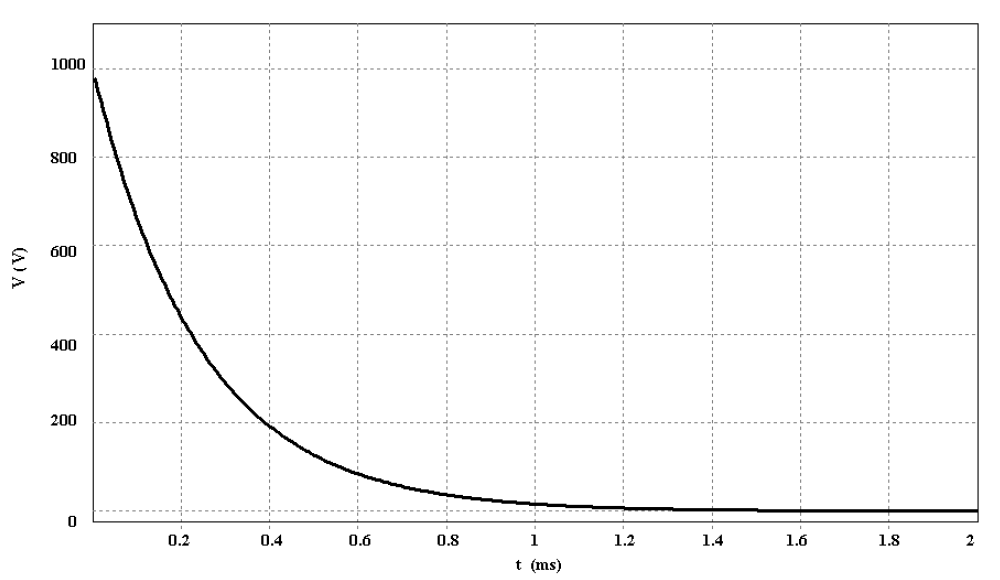
\includegraphics[width=16cm]{figuras/tensaoimpedanciahumana}}
% 		}{
% 			\Fonte{elaborado pelo autor (2016).}
% 		}	
% \end{figure}

% Texto texto texto texto texto texto texto texto texto texto texto texto texto texto texto texto texto texto texto texto texto texto texto texto texto texto texto texto texto texto texto texto texto texto texto texto texto texto texto texto texto texto texto texto texto texto texto texto texto texto texto texto texto texto texto texto texto texto texto texto texto texto texto texto texto texto texto texto texto.

% \begin{figure}[h!]
% 	\captionsetup{width=16cm}
% 	\Caption{\label{fig-grafico-1}Produção anual das dissertações de mestrado e teses de doutorado entre os anos de 1990 e 2008}		
% 	\IBGEtab{}{
% 		\fbox{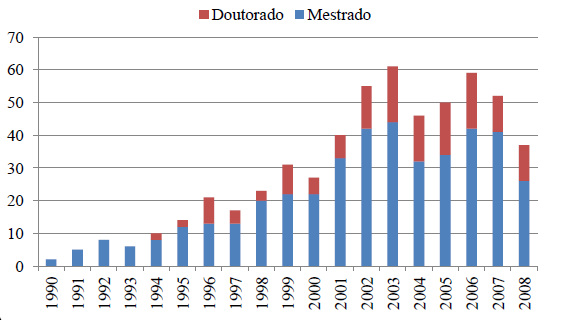
\includegraphics[width=16cm]{figuras/figura-3}}
% 	}{
% 	\Fonte{elaborado pelo autor (2016).}
% }
% \end{figure}

% Texto texto texto texto texto texto texto texto texto texto texto texto texto texto texto texto texto texto texto texto texto.

% Texto texto texto texto texto texto texto texto texto texto texto texto texto texto texto texto texto texto texto texto texto texto texto texto texto texto texto texto texto texto texto texto texto texto texto texto texto texto texto texto texto texto texto texto texto texto texto texto texto texto texto texto texto texto texto texto texto texto texto texto texto texto texto texto texto texto texto texto texto.

% \section{Resultados do Experimento B}
% \label{sec:resultados-do-experimento-b}

% Texto texto texto texto texto texto texto texto texto texto texto texto texto texto texto texto texto texto texto texto texto texto texto texto texto texto texto texto texto texto texto texto ..

% \begin{table}[h!]	
% 	%\centering
% 	\captionsetup{width=11.3cm}%ATENÇÃO: Ajuste a largura do título
% 	\Caption{\label{tab:notas} Notas dos participantes nas avaliações A, B e C}	
% 	\IBGEtab{}{
% 		\begin{tabular}{crrr}
% 			\toprule
% 			Identificação dos participantes & Avaliação A & Avaliação B &                        Avaliação C \\
% 			\midrule \midrule
% 			Participante 1 & 7 & 9 & 10\\
% 			Participante 2 & 8 & 2 & 1\\
% 			Participante 3 & 5 & 10 & 6 \\
% 			Participante 4 & 3 & 1 & 4\\
% 			Participante 5 & 2 & 4 & 1\\
% 			Participante 6 & 0 & 7 & 2\\
% 			\bottomrule
% 		\end{tabular}
% 	}{
% 	\Fonte{elaborado pelo autor (2016).}
% }
% \end{table}

%  Texto texto Referenciando a \autoref{tab:notas}  texto texto texto texto texto texto texto texto texto texto texto texto texto texto texto texto texto texto texto texto texto texto texto texto texto texto texto texto texto texto.Texto texto texto texto texto texto texto texto texto texto texto texto texto texto texto texto texto texto texto texto texto.

% Texto texto texto texto texto texto texto texto texto texto texto texto texto texto texto texto texto texto texto texto texto texto texto texto texto texto texto texto texto texto texto texto texto texto texto texto texto texto texto texto texto texto texto texto texto texto texto texto texto texto texto texto texto texto texto texto texto texto texto texto texto texto texto texto texto texto texto texto texto.Texto texto texto texto texto texto texto texto texto texto texto texto texto texto texto texto texto texto texto texto texto texto texto texto texto texto texto texto texto texto texto texto texto texto texto texto texto texto texto texto texto.

% Texto texto texto texto texto texto texto texto texto texto texto texto texto texto texto texto texto texto texto texto texto texto texto texto texto texto texto texto texto texto texto texto texto texto texto texto texto texto texto texto texto texto texto texto texto texto texto texto.Texto texto texto texto texto texto texto texto texto texto texto texto texto texto texto texto texto texto texto texto texto.

% Texto texto  Referenciando a \autoref{tab:notas}  texto texto texto texto texto texto texto texto texto texto texto texto texto texto texto texto texto texto texto texto texto texto texto texto texto texto texto texto texto texto texto texto texto texto texto texto texto texto texto texto texto texto texto texto texto texto texto texto texto texto texto texto texto texto texto texto texto texto texto texto texto texto texto texto texto texto texto.
	\chapter{Conclusões e Trabalhos Futuros}
\label{chap:conclusoes-e-trabalhos-futuros}

Parte final do texto na qual se apresentam as conclusões apoiadas no desenvolvimento do assunto. É a recapitulação sintética dos resultados obtidos. Pode apresentar recomendações e sugestões para pesquisas futuras.

%\label{sec:contribuicoes-do-trabalho}



%\label{sec:limitacoes}








	
	%Elementos pós-textuais	
	\bibliography{3-pos-textuais/referencias}
%	\imprimirglossario	
	\imprimirapendices
		% Adicione aqui os apendices do seu trabalho
		\apendice{Esquemático Eletrônico}
\label{ap:A}

Esquemático eletrônicos dos circuitos do hardware proposto.

%Código fonte para inserir um arquivo em PDF

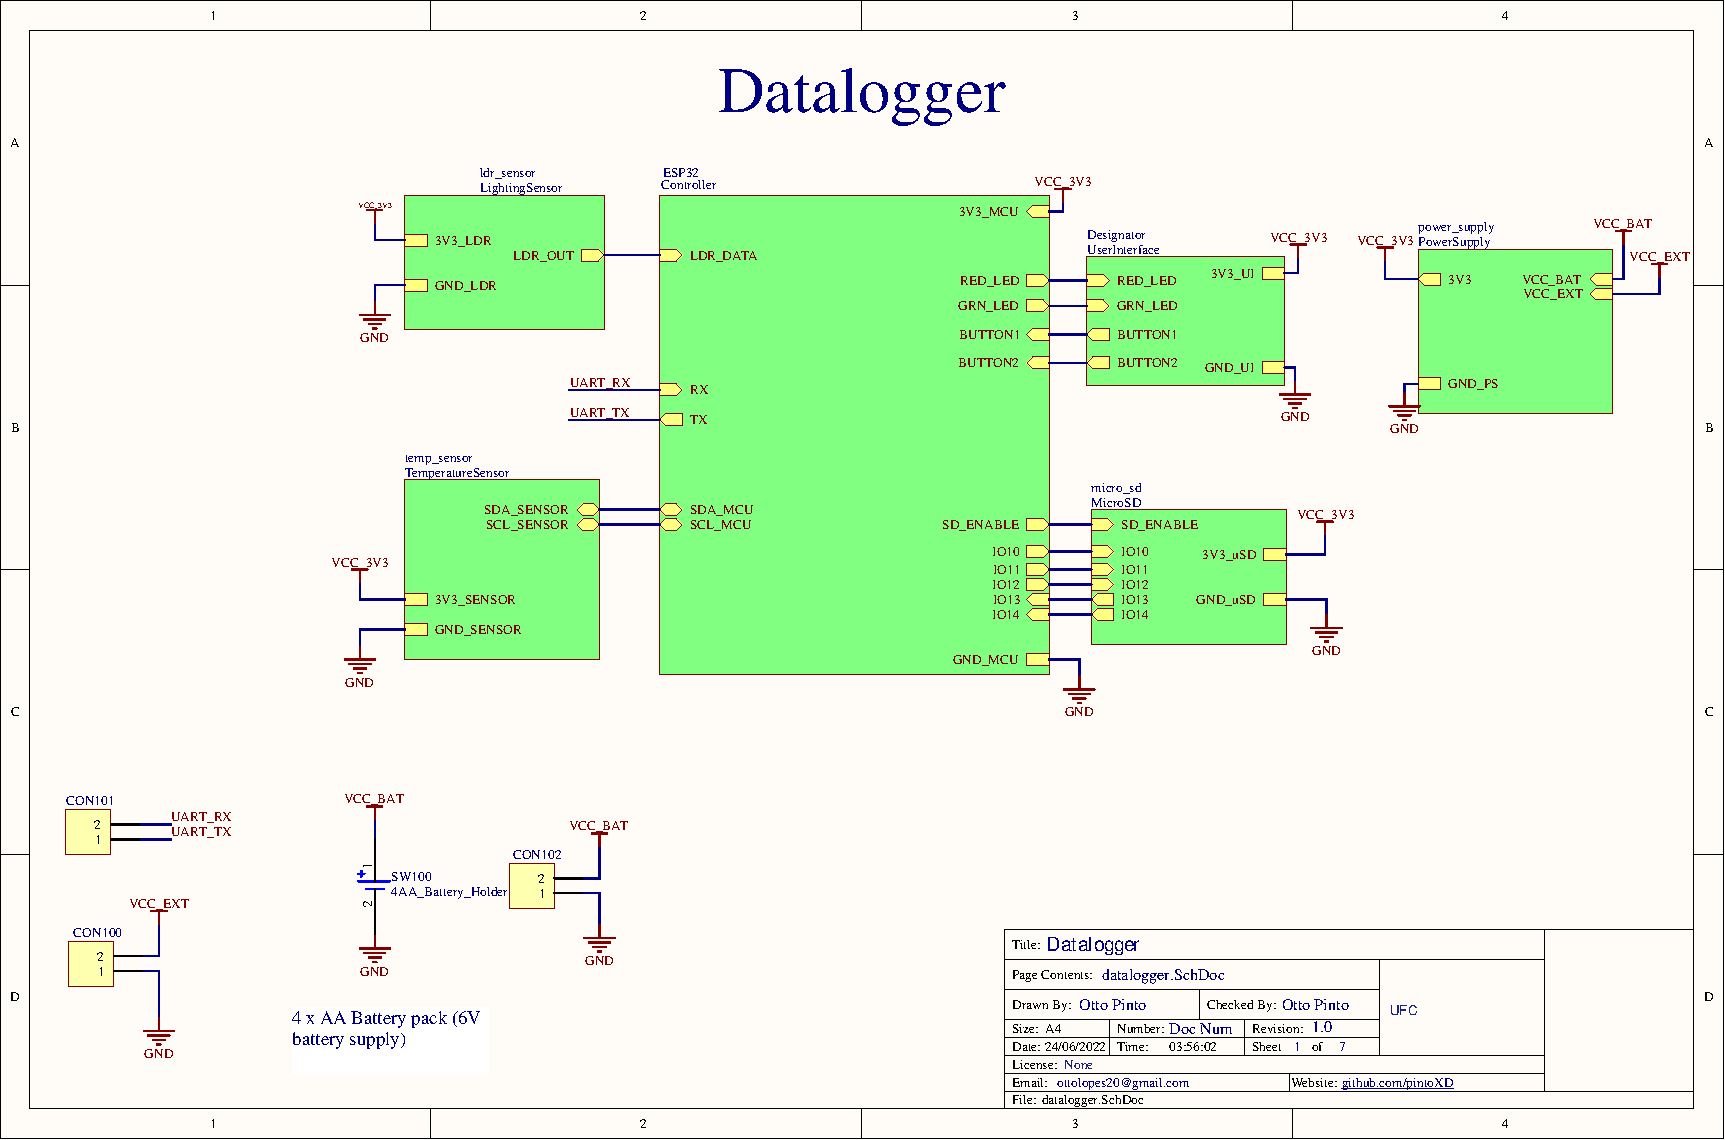
\includepdf[pages={1}, landscape=true, scale = 0.9]{3-pos-textuais/apendices/arquivos/Datalogger.PDF}

\includepdf[pages={2-7}, landscape=true, scale = 0.9]{3-pos-textuais/apendices/arquivos/Datalogger.PDF}


% Um apêndice é um documento elaborado pelo autor, diferentemente do anexo. Geralmente, se coloca como apêndice, questionários, códigos de programação, tabelas que tomariam muito espaço no meio do trabalho. Artigos, resumos ou qualquer publicação relacionada ao trabalho podem ser utilizados como apêndice.
		\apendice{Questionário utilizado para...}
\label{ap:B}

\begin{questao}
	\item Esta é a primeira questão com alguns itens:
		\begin{enumerate}
			\item Este é o primeiro item
			\item Segundo item
		\end{enumerate}
	\item Esta é a segunda questão:
		\begin{enumerate}
			\item Este é o primeiro item
			\item Segundo item
		\end{enumerate}
	\item Lorem ipsum dolor sit amet, consectetur adipiscing elit. Nunc dictum sed tortor nec viverra. consectetur adipiscing elit. Nunc dictum sed tortor nec viverra.
		\begin{enumerate}
			\item consectetur
			\item adipiscing
			\item Nunc
			\item dictum
		\end{enumerate}
\end{questao}

% 		\apendice{Códigos-fontes utilizados para...}
\label{ap:C}

\lstinputlisting[language=C++,caption={Hello World em C++}]{figuras/main.cpp}


\begin{lstlisting}[language=Java,caption={Hello World em Java}]
public class HelloWorld {
	public static void main(String[] args) {
		System.out.println("Hello World!");
	}
}
\end{lstlisting}


% 		\apendice{\textit{IEEE CEFC 2016}}
\label{ap:D}

\textit{Digest} submetido ao \textit{The 17th Biennial Conference on Eletromagnetic Field Computation, Miami FL - NOV 13-16, 2016, USA}.

%Código fonte para inserir um arquivo em PDF
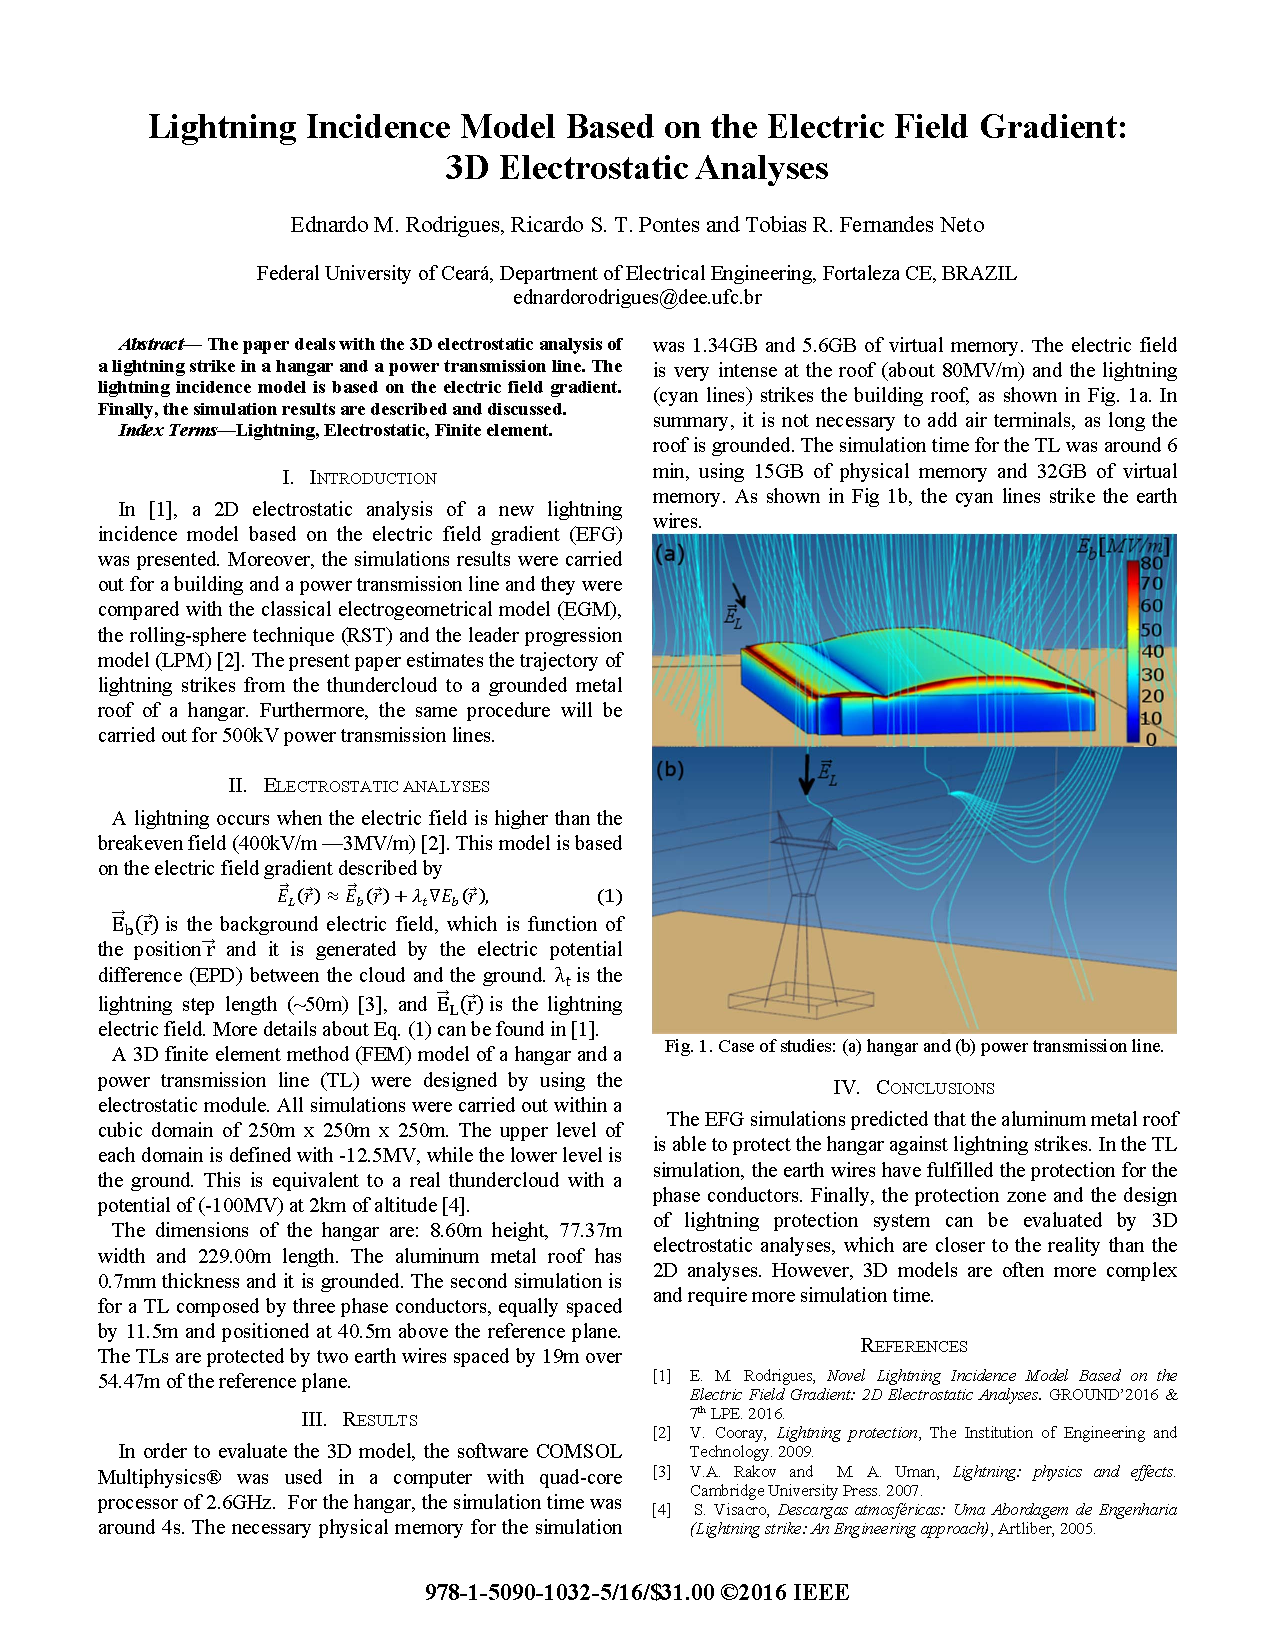
\includepdf[pages={-}]{3-pos-textuais/apendices/PID4416093.pdf}
	\imprimiranexos
		% Adicione aqui os anexos do seu trabalho
% 		\anexo{Exemplo de um anexo}
\label{an:ex_anexo_a}

Um anexo é um documento que não foi elaborado pelo autor, ou seja, o autor apenas anexa. Anexos podem ser tabelas, mapas, diagramas, \textit{datasheets}, manuais e etc. 




% 		\anexo{Exemplo de um anexo em PDF}
\label{an:ex_anexo_b}

O autor pode anexar um \gls{PDF}, traduzido como formato portátil de documento. Veja o código fonte utilizado para anexar o arquivo ``Sikasil.pdf'' que foi colocado dentro da pasta ``anexos'' que por sua vez está dentro da pasta ``elementos-pos-textuais''. Tenha muita atenção na hora de especificar o local do arquivo. Recomenda-se não utilizar caracteres especiais para nomear pastas e, principalmente, arquivos. 

Pode-se fazer uma descrição sucinta do arquivo anexado.

%Comando para incluir um arquivo em PDF:
% 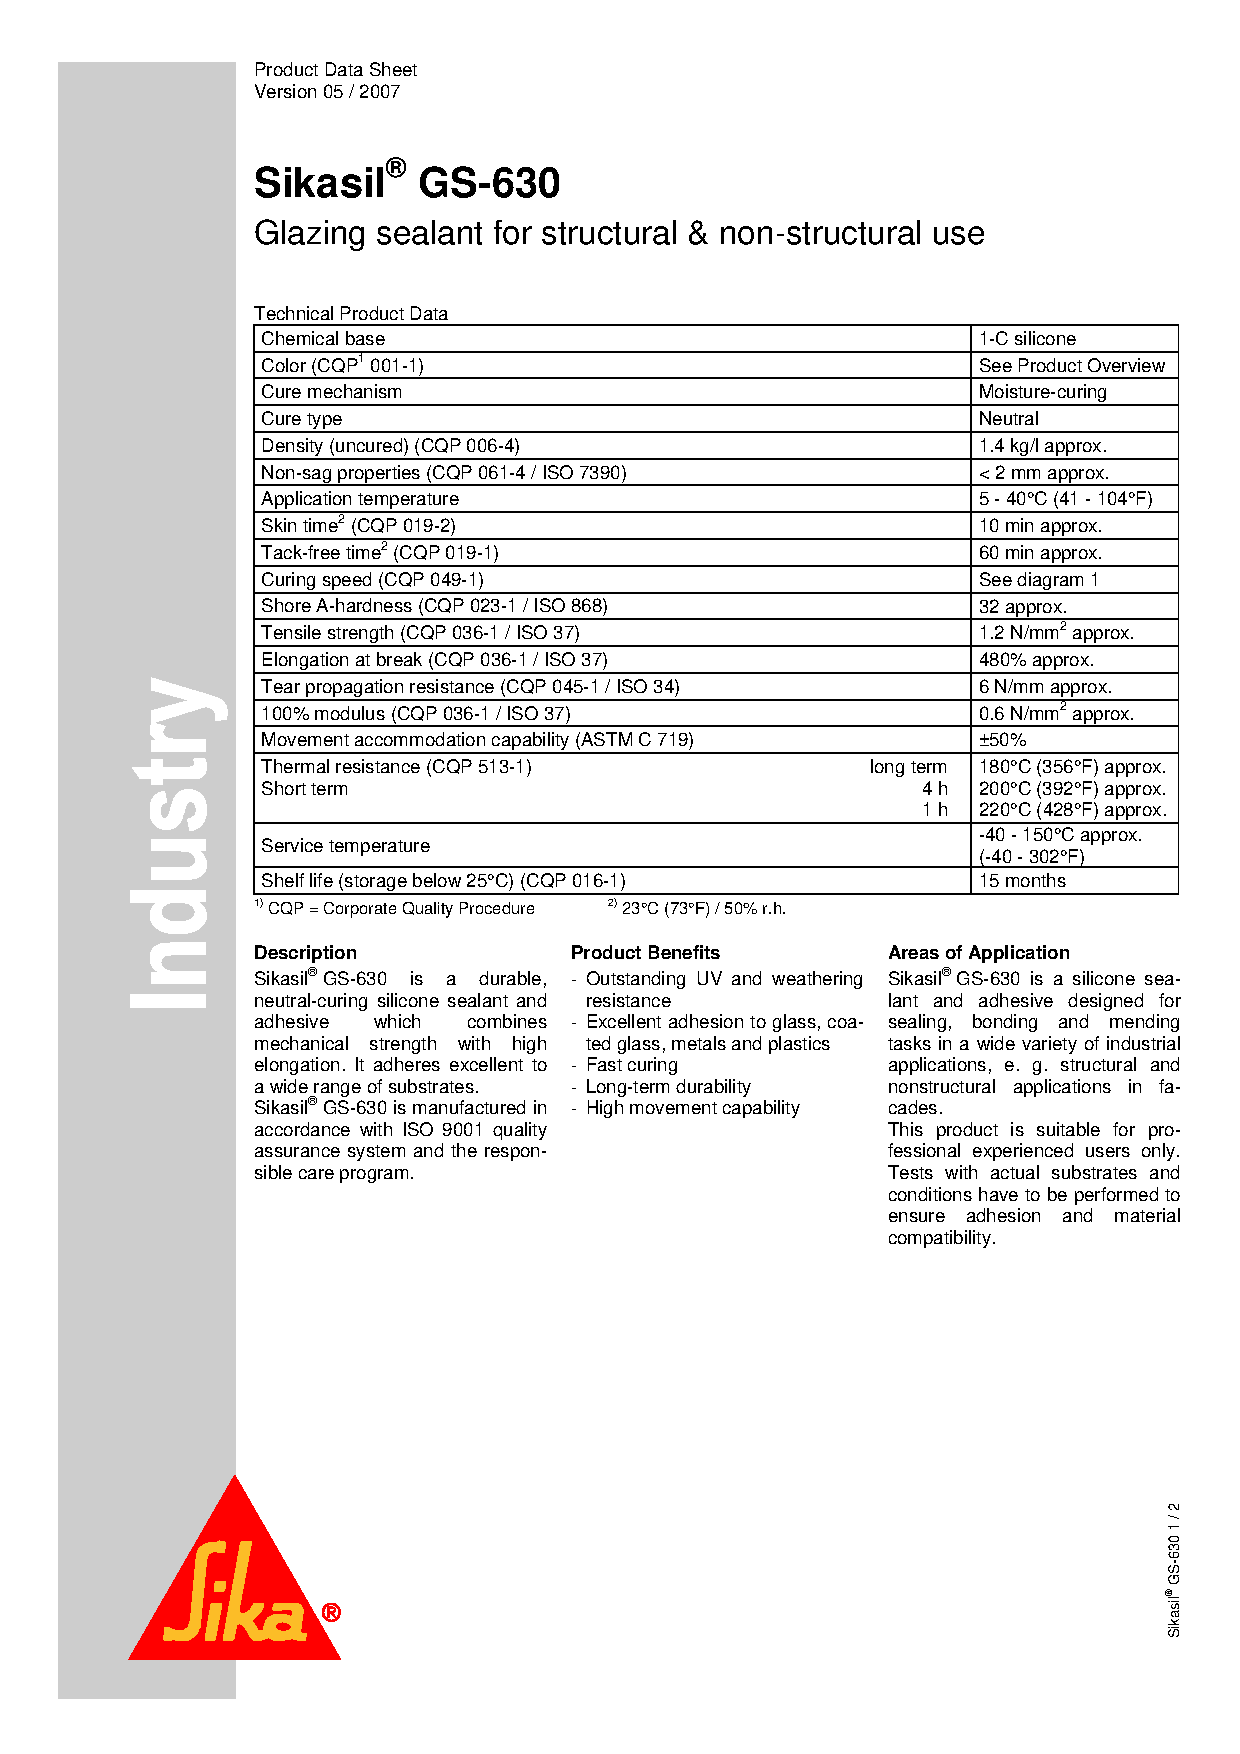
\includepdf[pages={-}]{3-pos-textuais/anexos/Sikasil.pdf}

		
	\imprimirindice

\end{document}